\documentclass[12pt,a4paper,oneside]{report}
\UseRawInputEncoding

% ===== Vietnamese + Encoding =====
\usepackage[T5]{fontenc}
\usepackage[utf8]{inputenc}
\usepackage[vietnamese]{babel}

% ===== Page layout & typography =====
\usepackage[a4paper,margin=2.5cm]{geometry}
\usepackage{setspace}
\onehalfspacing
\usepackage{microtype}
\setlength{\headheight}{18pt} % Fix fancyhdr warning
\usepackage{lmodern} % Latin Modern, scalable Computer Modern
% ===== Graphics, tables, math =====
\usepackage{graphicx}
\usepackage{float}
\usepackage{subcaption}
\usepackage{booktabs}
\usepackage{siunitx}
\sisetup{mode=match, propagate-math-font=true, round-mode=places, round-precision=2}
\usepackage{amsmath,amssymb,mathtools}

% ===== Lists & formatting =====
\usepackage{enumitem}
\setlist{noitemsep,leftmargin=2em}

% ===== TOC & Lists of figures/tables =====
\usepackage{tocloft}
\setlength{\cftbeforechapskip}{0.5em}
\renewcommand{\cftchapleader}{\cftdotfill{\cftdotsep}}

% ===== Hyperlinks & clever references =====
\usepackage{xcolor}
\definecolor{Link}{RGB}{0,0,128}
\definecolor{Cite}{RGB}{0,102,0}
\definecolor{URL}{RGB}{128,0,0}
\usepackage[
    unicode,
    pdfencoding=auto,
    colorlinks=true,
    linkcolor=Link,
    citecolor=Cite,
    urlcolor=URL
]{hyperref}
\usepackage{cleveref}

% ===== Header/Footer =====
\usepackage{fancyhdr}
\pagestyle{fancy}
\fancyhf{}
\lhead{\leftmark}
\rhead{\thepage}

% ===== Code listings (Python, JSON) =====
\usepackage{listings}
\lstdefinestyle{py}{
  language=Python,
  basicstyle=\ttfamily\footnotesize,
  numbers=left,
  numberstyle=\tiny,
  stepnumber=1,
  frame=single,
  breaklines=true
}
\lstdefinestyle{sql}{
  language=SQL,
  basicstyle=\ttfamily\footnotesize,
  numbers=left,
  numberstyle=\tiny,
  stepnumber=1,
  frame=single,
  breaklines=true
}
\lstdefinestyle{json}{
  language=,
  basicstyle=\ttfamily\footnotesize,
  numbers=left,
  numberstyle=\tiny,
  stepnumber=1,
  frame=single,
  breaklines=true
}

% ===== Glossaries / Acronyms (optional) =====
\usepackage[acronym]{glossaries}
\makeglossaries
\newacronym{apc}{APC}{Adaptive Phase Control}
\newacronym{rl}{RL}{Reinforcement Learning}
\newacronym{sumo}{SUMO}{Simulation of Urban MObility}
\newacronym{traci}{TraCI}{Traffic Control Interface}

% ===== Bibliography (biblatex with IEEE style) =====
\usepackage[backend=biber,style=ieee,sorting=none]{biblatex}
\addbibresource{reference.bib} % Đặt đúng tên file .bib

% ===== Title info =====
\title{\textbf{Hệ Thống Điều Khiển Đèn Giao Thông Thông Minh\\Dựa Trên Phương Pháp Lai APC và Học Tăng Cường}}
\author{Nguyễn Thái Sơn}
\date{\today}

\begin{document}
% ===== Title page =====
\maketitle

% ===== Front matter =====
\pagenumbering{roman}
\tableofcontents
\listoffigures
\listoftables

% ===== Danh mục từ viết tắt và thuật ngữ chuyên ngành =====
\addcontentsline{toc}{chapter}{Danh mục từ viết tắt và thuật ngữ chuyên ngành}

% In danh mục từ viết tắt (acronyms)
\printglossary[type=\acronymtype,title={Từ viết tắt phổ biến}]

% Danh sách thuật ngữ chuyên ngành
\section*{Thuật ngữ chuyên ngành}
\begin{description}[leftmargin=2.5em,style=nextline]
    \item[\textbf{Spillback}] Hiện tượng ùn tắc dội ngược: Khi hàng chờ tại một nút giao thông kéo dài vượt qua điểm đầu nút giao, làm cản trở hoặc chặn luôn dòng xe ở nút giao phía trước. Spillback gây ra hiệu ứng dây chuyền, lan rộng tắc nghẽn trong mạng lưới đô thị.
    \item[\textbf{Gridlock}] Kẹt lưới giao thông: Toàn bộ các nút giao đều bị kẹt, xe không thể di chuyển qua bất kỳ hướng nào do xung đột dòng xe cắt nhau.
    \item[\textbf{Starvation}] Đói phục vụ: Một làn hoặc hướng giao thông bị bỏ qua quá lâu, dẫn đến hàng chờ kéo dài không được phục vụ, thường xảy ra khi chính sách ưu tiên quá mức cho các hướng khác.
    \item[\textbf{Protected left}] Pha rẽ trái bảo vệ: Pha đèn tín hiệu được thiết kế riêng để cho phép rẽ trái an toàn, không bị xung đột với dòng đi thẳng đối diện.
    \item[\textbf{Adaptive Phase Control (APC)}] Điều khiển pha thích nghi: Phương pháp điều chỉnh thời lượng các pha đèn dựa trên trạng thái giao thông thực tế (hàng chờ, số xe dừng, v.v.).
    \item[\textbf{Reinforcement Learning (RL)}] Học tăng cường: Kỹ thuật học máy cho phép hệ thống điều khiển tín hiệu học từ phần thưởng/hình phạt dựa trên kết quả thực tế của hành động.
    \item[\textbf{Green wave}] Làn sóng xanh: Chuỗi các đèn tín hiệu được điều phối để xe chạy liên tục qua nhiều nút giao mà không phải dừng lại.
    \item[\textbf{Phase duration}] Thời lượng pha: Khoảng thời gian một pha đèn (xanh/vàng/đỏ) được duy trì trước khi chuyển sang pha tiếp theo.
    \item[\textbf{Supabase}] Nền tảng cơ sở dữ liệu đám mây, dùng lưu trữ trạng thái, nhật ký sự kiện và bảng Q-learning cho hệ thống điều khiển.
    \item[\textbf{SUMO}] Simulation of Urban Mobility: Phần mềm mô phỏng giao thông vi mô, dùng kiểm thử các thuật toán điều khiển tín hiệu.
    \item[\textbf{TraCI}] Traffic Control Interface: Giao thức kết nối giữa Python và SUMO, cho phép điều khiển và lấy dữ liệu mô phỏng theo thời gian thực.
    \item[\textbf{Q-table}] Bảng giá trị Q trong Q-learning: Lưu trữ giá trị kỳ vọng cho mỗi trạng thái và hành động, dùng để ra quyết định tối ưu cho agent học tăng cường.
    \item[\textbf{Pending requests}] Hàng đợi yêu cầu: Danh sách các yêu cầu chuyển pha đèn đang chờ xử lý, thường được xếp theo mức độ ưu tiên và thời gian.
\end{description}

% ===== Abstract =====
\chapter*{Tóm tắt}
\addcontentsline{toc}{chapter}{Tóm tắt}
Đèn giao thông đóng vai trò then chốt trong việc điều tiết lưu thông đô thị, song các hệ thống truyền thống thường thiếu khả năng thích ứng với biến động giao thông thực tế. Trong những năm gần đây, các phương pháp điều khiển thích nghi đã được nghiên cứu, nhưng vẫn còn tồn tại những hạn chế như hiện tượng nhấp nháy pha, xử lý tình huống khẩn cấp chưa hiệu quả và khó mở rộng cho nhiều nút giao.

Để khắc phục những vấn đề này, nghiên cứu đề xuất một bộ điều khiển nút giao thông thông minh được triển khai trên môi trường mô phỏng \gls{sumo}, kết nối qua \gls{traci}, kết hợp kỹ thuật học tăng cường và cơ chế lưu trữ trạng thái trên nền tảng đám mây Supabase. Bộ điều khiển có khả năng tự động điều chỉnh thời lượng đèn xanh dựa trên số lượng xe dừng, chiều dài hàng chờ và lưu lượng tức thời, đồng thời bảo đảm an toàn thông qua việc chèn pha vàng và duy trì tối thiểu thời gian đèn xanh.

Ngoài ra, hệ thống còn tích hợp cơ chế ưu tiên cho phương tiện khẩn cấp, quản lý ùn tắc và hỗ trợ rẽ trái an toàn thông qua hàng đợi yêu cầu có cấu trúc. Kết quả mô phỏng thực nghiệm cho thấy mô hình đề xuất giúp giảm đáng kể thời gian chờ trung bình và cải thiện lưu lượng so với phương pháp điều khiển tín hiệu cố định. Điều này chứng minh tính hiệu quả, linh hoạt và tiềm năng ứng dụng của hệ thống trong quản lý giao thông đô thị thông minh.

\clearpage
\pagenumbering{arabic}

% =========================
% CHƯƠNG 1
% =========================
% =========================
% CHƯƠNG 1
% =========================
\chapter{Tổng quan dự án}

\section{Giới thiệu dự án}
Trong bối cảnh đô thị hóa nhanh chóng, các thành phố lớn ngày càng đối mặt với tình trạng ùn tắc giao thông nghiêm trọng. Sự gia tăng đột biến của phương tiện cá nhân, kết hợp với tốc độ mở rộng hạ tầng giao thông chưa theo kịp, đã tạo ra những áp lực lớn đối với hệ thống điều tiết lưu lượng. Ùn tắc không chỉ gây ra sự lãng phí thời gian mà còn kéo theo nhiều hệ quả tiêu cực khác như tiêu hao nhiên liệu, phát thải khí thải nhà kính, gia tăng ô nhiễm môi trường và ảnh hưởng xấu đến sức khỏe cộng đồng. Bên cạnh đó, các tình huống khẩn cấp như xe cứu thương, cứu hỏa hoặc cảnh sát gặp khó khăn khi di chuyển qua các nút giao đông đúc càng làm bộc lộ hạn chế của hệ thống điều khiển tín hiệu hiện tại.

Các hệ thống đèn tín hiệu giao thông truyền thống thường được lập trình dựa trên chu kỳ cố định, được xác định sẵn từ dữ liệu trung bình lịch sử. Tuy nhiên, phương pháp này thiếu tính linh hoạt, không thể thích ứng kịp thời với biến động lưu lượng thực tế vốn thay đổi liên tục theo thời gian, vị trí và điều kiện giao thông. Kết quả là ở những hướng có mật độ phương tiện thấp, thời gian đèn xanh bị lãng phí, trong khi ở những hướng có lưu lượng cao lại hình thành hàng chờ dài và ùn tắc kéo dài. Sự cứng nhắc này khiến hiệu quả vận hành của mạng lưới giao thông giảm đáng kể và đặt ra yêu cầu cấp bách về một giải pháp điều khiển tín hiệu thông minh, thích ứng theo thời gian thực.

Để giải quyết vấn đề trên, dự án này phát triển một \textbf{hệ thống điều khiển đèn giao thông thông minh}, kết hợp giữa \textbf{điều khiển pha thích nghi (Adaptive Phase Control – APC)} và \textbf{học tăng cường (Reinforcement Learning – RL)}. APC cung cấp nền tảng điều khiển theo luật, cho phép điều chỉnh độ dài pha đèn dựa trên các ngưỡng hàng chờ hoặc số lượng xe dừng. Trong khi đó, RL mang lại khả năng học hỏi từ trải nghiệm, tối ưu dần chiến lược điều khiển thông qua cơ chế phần thưởng – hình phạt, giúp hệ thống thích nghi linh hoạt hơn với các tình huống giao thông phức tạp.

Hệ thống được kiểm thử trong môi trường mô phỏng \textbf{SUMO}, kết nối thông qua \textbf{TraCI}, đồng thời tích hợp \textbf{Supabase} để lưu trữ và đồng bộ dữ liệu trên nền tảng đám mây. Cách tiếp cận này không chỉ cho phép đánh giá hiệu năng của bộ điều khiển trong các kịch bản đa dạng mà còn mở ra khả năng mở rộng sang quy mô thực tế, hỗ trợ phân tích dữ liệu dài hạn và triển khai trong các hệ thống giao thông đô thị thông minh trong tương lai.

\section{Thành tựu chính}
\begin{itemize}
    \item Xây dựng bộ điều khiển lai \textbf{APC–RL} điều chỉnh chu kỳ đèn theo trạng thái giao thông.
    \item Cơ chế \textbf{ưu tiên phương tiện khẩn cấp}.
    \item Thuật toán \textbf{phát hiện và xử lý tắc nghẽn} (giảm spillback).
    \item \textbf{Rẽ trái bảo vệ} với pha bảo vệ động.
    \item Kết nối Supabase để \textbf{sao lưu trạng thái} và phân tích.
\end{itemize}

\section{Tóm tắt cải thiện hiệu năng}
Theo nghiên cứu của Eom và Kim \cite{Eom2020}, các hệ thống điều khiển tín hiệu thích nghi có thể cải thiện đáng kể hiệu suất giao thông. Kết quả thực nghiệm của dự án này cho thấy:

\begin{itemize}
    \item \textbf{Điều chỉnh pha:} trung bình +13.9s (kéo dài 87.1\%, rút ngắn 10.4\%), tối đa +88s / $-70$s.
    \item \textbf{Thời gian chờ:} giảm từ \textbf{2061.5s} (mặc định) xuống \textbf{1412.7s} (APC–RL) $\Rightarrow$ \textbf{-31.5\%}.
    \item \textbf{Hàng chờ:} 49.1 xe (APC–RL) so với 51.6 xe (mặc định).
    \item \textbf{Tốc độ trung bình:} 1.2 m/s (APC–RL) vs 0.8 m/s (mặc định).
\end{itemize}

\section{Tổng quan công nghệ sử dụng} 
Hệ thống điều khiển được xây dựng dựa trên sự tích hợp của nhiều công nghệ phần mềm và công cụ mô phỏng, đảm bảo khả năng xử lý dữ liệu thời gian thực, học tăng cường và trực quan hóa kết quả. Cụ thể: 
\begin{itemize} 
  \item \textbf{SUMO (Simulation of Urban MObility)}: công cụ mô phỏng giao thông mã nguồn mở, dùng để xây dựng mạng lưới đường phố, luồng xe, và kiểm thử các chiến lược điều khiển tín hiệu. 
   \item \textbf{TraCI (Traffic Control Interface)}: giao thức cầu nối giữa Python và SUMO, cho phép điều khiển đèn tín hiệu theo từng bước thời gian, lấy dữ liệu trạng thái như độ dài hàng chờ, thời gian chờ, tốc độ xe.
    \item \textbf{Python}: ngôn ngữ lập trình chính của hệ thống. Các thành phần quan trọng bao gồm: 
    \begin{itemize} 
      \item Bộ điều khiển pha thích nghi (Adaptive Phase Controller - APC) với logic tính toán thời lượng pha. 
      \item Agent Q-learning tăng cường (Enhanced Q-Learning Agent) cho việc ra quyết định tối ưu dựa trên trạng thái giao thông.
      \item Bộ quản lý vòng lặp chính để phối hợp giữa hai thành phần trên (hybrid APC–RL).
    \end{itemize} 
    \item \textbf{Supabase}: nền tảng cơ sở dữ liệu đám mây, được dùng để lưu trữ bảng Q-learning (Q-table), nhật ký các sự kiện điều khiển, dữ liệu trạng thái giao thông, đồng thời hỗ trợ đồng bộ dữ liệu trong thời gian thực.
    \item \textbf{Các thư viện Python hỗ trợ}:
    \begin{itemize} 
      \item \texttt{NumPy} và \texttt{Pandas} cho xử lý ma trận trạng thái, dữ liệu hàng chờ và tính toán thống kê. 
       \item \texttt{Matplotlib} để trực quan hóa kết quả mô phỏng: hàng chờ, thời gian chờ, tốc độ trung bình và phân tích điều chỉnh pha. 
       \item \texttt{Supabase-py} để kết nối và quản lý dữ liệu đám mây.
       \item \texttt{Pickle} dùng lưu trữ/tải lại bảng Q-learning dưới dạng file nhị phân. \end{itemize} 
    \end{itemize}


% =========================
% CHƯƠNG 2
% =========================
% =========================
% CHƯƠNG 2 - GIỚI THIỆU
% =========================
\chapter{Giới thiệu}

\section{Bài toán nghiên cứu}

\subsection{Tác động của ùn tắc giao thông đô thị}
Ùn tắc giao thông là vấn đề phổ biến tại các trung tâm đô thị, gây tổn thất về thời gian, nhiên liệu và môi trường, đồng thời giảm chất lượng dịch vụ giao thông. Sự biến động theo thời gian và không đồng đều giữa các hướng khiến các giải pháp cố định khó đáp ứng được yêu cầu thực tế, đặc biệt trong giờ cao điểm hoặc khi xuất hiện sự kiện bất thường.

\subsection{Giới hạn của điều khiển thời gian cố định}
Các hệ thống điều khiển tín hiệu truyền thống dựa trên chu kỳ cố định (fixed‑time) thường được thiết kế theo mẫu lưu lượng trung bình. Nhược điểm chính là thiếu khả năng thích ứng với biến động thực tế: khi lưu lượng giảm, thời gian xanh có thể bị lãng phí; khi lưu lượng tăng, hàng chờ dễ hình thành và kéo dài. Các phương pháp semi/fully‑actuated cải thiện phần nào nhưng vẫn bị hạn chế bởi các tham số cố định và khả năng tối ưu trên mạng lưới lớn.

\subsection{Yêu cầu ưu tiên cho phương tiện khẩn cấp}
Một yêu cầu thiết yếu trong quản lý tín hiệu là đảm bảo phục vụ phương tiện ưu tiên (xe cứu thương, cứu hỏa, cảnh sát). Hệ thống cần phát hiện kịp thời và điều chỉnh pha sao cho phương tiện ưu tiên được thông suốt, đồng thời giảm thiểu tác động tiêu cực lên lưu lượng chung.

\subsection{Vấn đề rẽ trái và xung đột pha}
Xung đột giữa luồng rẽ trái và luồng đi thẳng đối diện là nguyên nhân phổ biến dẫn tới tắc nghẽn cục bộ và nguy cơ tai nạn. Thiết kế pha rẽ trái cố định thường không linh hoạt khi điều kiện thay đổi, do đó cần cơ chế phát hiện rẽ trái bị chặn và tạo pha bảo vệ động để giải phóng luồng.

\section{Mục tiêu nghiên cứu}

Mục tiêu chính của luận văn là phát triển một hệ thống điều khiển đèn giao thông lai, kết hợp bộ điều khiển pha thích nghi (APC) với học tăng cường (RL), nhằm:
\begin{itemize}
    \item Tăng khả năng thích ứng với biến động lưu lượng thời gian thực,
    \item Giảm thời gian chờ trung bình và độ dài hàng chờ,
    \item Hỗ trợ ưu tiên phương tiện khẩn cấp và xử lý rẽ trái bị chặn,
    \item Đảm bảo tính an toàn (chèn pha vàng, ngăn xung đột) và khả năng phục hồi khi mất kết nối với hệ thống lưu trữ.
\end{itemize}

\section{Phạm vi và giới hạn}

Công trình được thực nghiệm trong môi trường mô phỏng SUMO và tập trung chính vào tối ưu cho một nút giao hoặc cụm nút nhỏ. Những giới hạn chính bao gồm:
\begin{itemize}
    \item Sử dụng Q‑learning rời rạc cho tác tử RL (chưa triển khai Deep RL cho không gian trạng thái liên tục).
    \item Kết quả dựa trên dữ liệu mô phỏng; việc chuyển sang triển khai thực tế (sim‑to‑real) yêu cầu bổ sung domain randomization và tích hợp cảm biến thực.
    \item Khả năng điều phối đa nút ở mức sơ khai; cần mở rộng thêm để xử lý mạng lưới lớn với độ trễ giao tiếp thực.
\end{itemize}

\section{Đóng góp chính}

Luận văn đóng góp những điểm chính sau:
\begin{itemize}
    \item Mô hình lai APC–RL kết hợp quy tắc an toàn và cơ chế học để điều chỉnh thời lượng pha theo reward đa mục tiêu.
    \item Cơ chế quản lý yêu cầu ưu tiên (pending requests) cho phép phục vụ xe khẩn cấp, starvation và congestion theo thứ tự ưu tiên.
    \item Kiến trúc lưu trữ lai (local pickle cho Q‑table và Supabase cho log/state) đảm bảo khả năng tái tạo, phân tích và phục hồi.
    \item Bộ công cụ đánh giá trong SUMO cho phép so sánh với baseline fixed‑time và phân tích các kịch bản congestion, priority và blocked left.
\end{itemize}

\section{Cấu trúc chương tiếp theo}
Tài liệu được tổ chức như sau:
\begin{itemize}
    \item Chương 3: Tổng quan tài liệu liên quan và khoảng trống nghiên cứu.
    \item Chương 4–7: Thiết kế hệ thống, APC, thành phần RL và chiến lược điều khiển lai.
    \item Chương 8–10: Quản lý phương tiện ưu tiên, quản lý dữ liệu và chi tiết triển khai.
    \item Chương 11–13: Thiết lập thí nghiệm, đánh giá hiệu năng và thảo luận kết quả.
    \item Chương 14–16: Trực quan hóa, hướng phát triển tương lai và kết luận.
\end{itemize}

% =========================
% CHƯƠNG 3
% =========================

% =========================
% CHƯƠNG 3
% =========================
\chapter{Tổng quan tài liệu}
\section{Các phương pháp điều khiển giao thông truyền thống}

Hệ thống điều khiển tín hiệu giao thông truyền thống thường dựa trên hai phương pháp chính: điều khiển theo chu kỳ cố định (fixed-time control) và điều khiển kích hoạt (actuated control) \cite{Papageorgiou2003, Eom2020}. 

\subsection{Điều khiển chu kỳ cố định}

Hệ thống điều khiển chu kỳ cố định hoạt động dựa trên các chu trình tín hiệu được xác định trước, tính toán từ dữ liệu giao thông lịch sử. Phương pháp này thường sử dụng các công thức tối ưu hóa như phương pháp Webster để xác định độ dài chu kỳ và phân chia thời gian cho các pha tín hiệu \cite{Webster1958, Urbanik2015, Shingate2020}. 

Ưu điểm của hệ thống cố định bao gồm:
\begin{itemize}
    \item Thiết kế đơn giản, dễ triển khai và bảo trì
    \item Chi phí đầu tư và vận hành thấp
    \item Độ tin cậy cao do không phụ thuộc vào cảm biến
    \item Được áp dụng rộng rãi trên toàn cầu
\end{itemize}

Tuy nhiên, phương pháp này tồn tại những hạn chế đáng kể:
\begin{itemize}
    \item Thiếu khả năng thích ứng với biến động giao thông thời gian thực
    \item Thường xuyên xảy ra hiện tượng lãng phí thời gian đèn xanh khi lưu lượng thấp
    \item Hình thành hàng chờ dài trong giờ cao điểm hoặc khi có sự kiện bất thường
    \item Không thể xử lý hiệu quả các tình huống khẩn cấp hoặc sự cố giao thông
\end{itemize}

Những hạn chế này đã được nhiều nghiên cứu chỉ ra và phân tích chi tiết \cite{Zhao2012, Shaikh2022}.

\subsection{Điều khiển kích hoạt}

Điều khiển kích hoạt (actuated control) sử dụng các cảm biến phát hiện phương tiện để điều chỉnh thời gian tín hiệu trong phạm vi giới hạn định trước. Hệ thống này có thể kéo dài pha đèn xanh khi phát hiện còn nhiều phương tiện hoặc chuyển pha sớm khi không có nhu cầu \cite{Koonce2008, Eom2020}.

Các dạng điều khiển kích hoạt bao gồm:
\begin{itemize}
    \item \textbf{Semi-actuated control}: Chỉ lắp cảm biến trên các hướng phụ, hướng chính luôn được ưu tiên
    \item \textbf{Fully-actuated control}: Tất cả các hướng đều có cảm biến, thời gian tín hiệu được điều chỉnh linh hoạt theo nhu cầu thực tế
\end{itemize}

Mặc dù linh hoạt hơn điều khiển cố định, phương pháp kích hoạt vẫn bị giới hạn bởi các tham số định trước và không thể tối ưu hóa toàn diện cho mạng lưới giao thông \cite{Mirchandani2001}.

\subsection{Điều khiển phối hợp}

Ngoài hai phương pháp trên, điều khiển phối hợp (coordinated control) đồng bộ hóa tín hiệu giữa nhiều nút giao liên tiếp để tạo "làn sóng xanh", giúp phương tiện di chuyển liên tục qua nhiều giao lộ mà không phải dừng lại \cite{Hunt1981, Lowrie1990}. Hai hệ thống phối hợp nổi tiếng nhất là SCOOT (Split Cycle Offset Optimisation Technique) \cite{Hunt1981} và SCATS (Sydney Coordinated Adaptive Traffic System) \cite{Lowrie1990}. Phương pháp này đặc biệt hiệu quả trên các trục đường chính nhưng đòi hỏi thiết kế phức tạp và khó điều chỉnh khi mạng lưới giao thông có nhiều hướng với lưu lượng cân bằng.

\subsection{Đánh giá chung}

Mặc dù các phương pháp truyền thống đã được triển khai rộng rãi và chứng minh hiệu quả trong nhiều trường hợp, chúng vẫn không đáp ứng được yêu cầu ngày càng cao của giao thông đô thị hiện đại. Sự thiếu linh hoạt trong việc thích ứng với điều kiện giao thông động và phức tạp đã thúc đẩy sự phát triển của các hệ thống điều khiển thích nghi và thông minh hơn, đặc biệt là các phương pháp dựa trên học máy và trí tuệ nhân tạo \cite{Abdulhai2003, Li2016, Shaikh2022}.

\section{Hệ thống điều khiển giao thông thích nghi}
Các hệ thống thích nghi như SCOOT, SCATS và OPAC đã được phát triển để khắc phục hạn chế của hệ thống cố định \cite{Eom2020}. Những hệ thống này có khả năng điều chỉnh thời gian tín hiệu dựa trên điều kiện giao thông thực tế.

\section{Ứng dụng học tăng cường trong quản lý giao thông}
Học tăng cường đã cho thấy tiềm năng lớn trong việc tối ưu hóa điều khiển tín hiệu giao thông thông qua khả năng học từ tương tác với môi trường \cite{Eom2020}.

\section{Phương pháp lai trong điều khiển tín hiệu}
Việc kết hợp nhiều phương pháp điều khiển có thể tận dụng ưu điểm của từng cách tiếp cận, tạo ra hệ thống hiệu quả hơn \cite{Eom2020}.

\section{Phân tích khoảng trống nghiên cứu}

Mặc dù đã có nhiều nghiên cứu về điều khiển tín hiệu giao thông thích nghi và ứng dụng học máy, vẫn tồn tại nhiều khoảng trống quan trọng cần được giải quyết để phát triển hệ thống điều khiển có khả năng ứng dụng thực tế cao.

\subsection{Hạn chế về khả năng mở rộng của thuật toán học tăng cường}

Phần lớn các nghiên cứu hiện tại sử dụng Q-learning với bảng Q rời rạc \cite{Watkins1992, Mannion2016}, phù hợp cho không gian trạng thái và hành động nhỏ. Tuy nhiên, trong môi trường giao thông thực tế với không gian trạng thái lớn và liên tục, phương pháp này gặp phải các hạn chế nghiêm trọng:

\begin{itemize}
    \item \textbf{Thiếu khả năng khái quát hóa}: Không có hàm xấp xỉ như mạng nơ-ron sâu để tổng quát hóa cho các trạng thái chưa từng gặp, dẫn đến khó khăn trong việc mở rộng sang mạng lưới giao thông lớn \cite{Li2016, Liang2019}.
    
    \item \textbf{Biểu diễn trạng thái hạn chế}: Vector trạng thái thường được thiết kế đơn giản, thiếu thông tin về topology mạng, tương tác đa nút và đặc trưng thời gian dài hạn \cite{Wei2019}.
    
    \item \textbf{Nguy cơ overfitting}: Tác tử có thể bị quá khớp với kịch bản mô phỏng cụ thể và không chuyển giao tốt sang môi trường thực tế \cite{Gao2017}.
\end{itemize}

\subsection{Thiếu phương pháp đánh giá chuẩn và kiểm chứng thống kê}

Nhiều nghiên cứu chưa thiết lập quy trình đánh giá khoa học chặt chẽ:

\begin{itemize}
    \item \textbf{Thiếu benchmark chuẩn}: Không có so sánh hệ thống với các baseline phổ biến như SCOOT, SCATS hoặc các phương pháp RL hiện đại (DQN, PPO, A2C) trên cùng bộ dữ liệu \cite{Hunt1981, Lowrie1990}.
    
    \item \textbf{Kiểm chứng thống kê yếu}: Thiếu thủ tục thống kê nghiêm ngặt như chạy nhiều lần với seed khác nhau, tính confidence intervals, và thực hiện kiểm định t-test để xác nhận ý nghĩa thống kê của kết quả \cite{Shaikh2022}.
    
    \item \textbf{Đánh giá không toàn diện}: Chỉ tập trung vào một số metrics cơ bản mà bỏ qua các khía cạnh quan trọng như độ ổn định, khả năng thích ứng với biến động \cite{Zhao2020}.
\end{itemize}

\subsection{Hạn chế trong điều phối đa nút và khả năng mở rộng}

Vấn đề phối hợp giữa nhiều nút giao thông vẫn chưa được giải quyết triệt để:

\begin{itemize}
    \item \textbf{Thiếu cơ chế phối hợp phân tán}: Các nghiên cứu thường tập trung vào tối ưu đơn nút, thiếu giải pháp cho multi-agent coordination với kiến trúc CTDE (Centralized Training, Decentralized Execution) \cite{Kouvelas2011}.
    
    \item \textbf{Khả năng mở rộng hạn chế}: Chưa có thử nghiệm trên mạng lưới lớn (hàng chục đến hàng trăm nút) với xem xét về độ trễ giao tiếp, overhead tính toán \cite{Zhao2012}.
    
    \item \textbf{Topology động}: Thiếu nghiên cứu về khả năng thích ứng khi topology mạng thay đổi do sự cố hoặc điều chỉnh hạ tầng.
\end{itemize}

\subsection{Khoảng cách giữa mô phỏng và thực tế (Sim-to-Real Gap)}

Việc chuyển giao từ môi trường mô phỏng sang thực tế vẫn là thách thức lớn:

\begin{itemize}
    \item \textbf{Thiếu domain randomization}: Các mô hình không được huấn luyện với biến động về sensor noise, mất gói tin, độ trễ mạng \cite{Lopez2018}.
    
    \item \textbf{Phụ thuộc vào mô phỏng}: Hiệu năng phụ thuộc nhiều vào độ chính xác của mô phỏng SUMO, thiếu kiểm thử trên nhiều môi trường mô phỏng khác nhau.
    
    \item \textbf{Thiếu tích hợp thực tế}: Chưa có nghiên cứu về kết nối với cảm biến thực, hệ thống V2X hoặc camera giao thông thực tế.
\end{itemize}

\subsection{Thiếu sót trong thiết kế hàm thưởng và phân tích bias}

Hàm thưởng trong RL thường được thiết kế phức tạp nhưng thiếu phân tích sâu:

\begin{itemize}
    \item \textbf{Reward shaping không rõ ràng}: Thiếu phân tích về cách các thành phần reward ảnh hưởng đến hành vi học, có thể dẫn đến các bias không mong muốn \cite{Sutton2018}.
    
    \item \textbf{Thiếu ablation study}: Không có nghiên cứu tách biệt để đánh giá tác động của từng thành phần trong hàm thưởng.
    
    \item \textbf{Vấn đề công bằng}: Khó đảm bảo công bằng giữa các hướng giao thông khi tối ưu hóa đa mục tiêu.
\end{itemize}

\subsection{Thiếu cơ chế đảm bảo an toàn và ràng buộc cứng}

An toàn là yếu tố then chốt nhưng thường bị bỏ qua:

\begin{itemize}
    \item \textbf{Thiếu chứng minh hình thức}: Không có cơ chế verification để đảm bảo hệ thống không vi phạm các ràng buộc an toàn cơ bản \cite{Mirchandani2001}.
    
    \item \textbf{Kiểm thử stress hạn chế}: Thiếu thử nghiệm với các corner cases, gridlock cực đoan, hoặc sự cố hệ thống.
    
    \item \textbf{Xung đột pha}: Chưa có giải pháp triệt để cho việc đảm bảo không xảy ra xung đột pha nguy hiểm.
\end{itemize}

\subsection{Hiệu quả mẫu và tốc độ hội tụ}

Các thuật toán học tăng cường truyền thống yêu cầu lượng dữ liệu huấn luyện lớn:

\begin{itemize}
    \item \textbf{Sample inefficiency}: Q-learning cơ bản yêu cầu số lượng lớn episodes để hội tụ, không phù hợp cho học online \cite{Watkins1992}.
    
    \item \textbf{Thiếu kỹ thuật tăng cường}: Không áp dụng experience replay, prioritized replay, hoặc model-based RL để cải thiện hiệu quả mẫu \cite{Gao2017}.
    
    \item \textbf{Thời gian huấn luyện}: Thiếu báo cáo về thời gian và tài nguyên tính toán cần thiết cho quá trình học.
\end{itemize}

\subsection{Thiếu khả năng tái tạo và minh bạch}

Nhiều nghiên cứu không cung cấp đủ thông tin để tái tạo kết quả:

\begin{itemize}
    \item \textbf{Tham số không rõ ràng}: Thiếu documentation về hyperparameters, random seeds, cấu hình chi tiết \cite{Shaikh2022}.
    
    \item \textbf{Code không công khai}: Nhiều nghiên cứu không chia sẻ mã nguồn, khiến việc verify và so sánh trở nên khó khăn.
    
    \item \textbf{Dữ liệu không chuẩn}: Sử dụng các bộ dữ liệu riêng biệt, không có benchmark dataset chung cho cộng đồng.
\end{itemize}

\subsection{Kết luận về khoảng trống nghiên cứu}

Những khoảng trống trên cho thấy cần có một cách tiếp cận tổng hợp, kết hợp ưu điểm của điều khiển dựa trên luật (rule-based) với khả năng học và thích ứng của học máy, đồng thời đảm bảo tính an toàn, khả năng mở rộng và ứng dụng thực tế. Nghiên cứu này hướng đến việc giải quyết một phần các khoảng trống quan trọng thông qua việc phát triển hệ thống điều khiển lai APC--RL với các cơ chế an toàn, quản lý ưu tiên và khả năng đồng bộ dữ liệu thời gian thực, tạo nền tảng cho các nghiên cứu mở rộng trong tương lai.
% =========================
% CHƯƠNG 4
% =========================
% =========================
% CHƯƠNG 4
% =========================
\chapter{Kiến trúc hệ thống}

\section{Thiết kế tổng thể}

Hệ thống điều khiển đèn giao thông thông minh được thiết kế theo mô hình phân tầng, kết hợp giữa điều khiển dựa trên luật (rule-based) và học máy (machine learning). Kiến trúc này cho phép hệ thống vừa đảm bảo tính ổn định, an toàn thông qua các quy tắc cứng, vừa có khả năng thích ứng và tối ưu hóa thông qua học tăng cường.

\subsection{Sơ đồ thành phần hệ thống}

\begin{figure}[H]
    \centering
    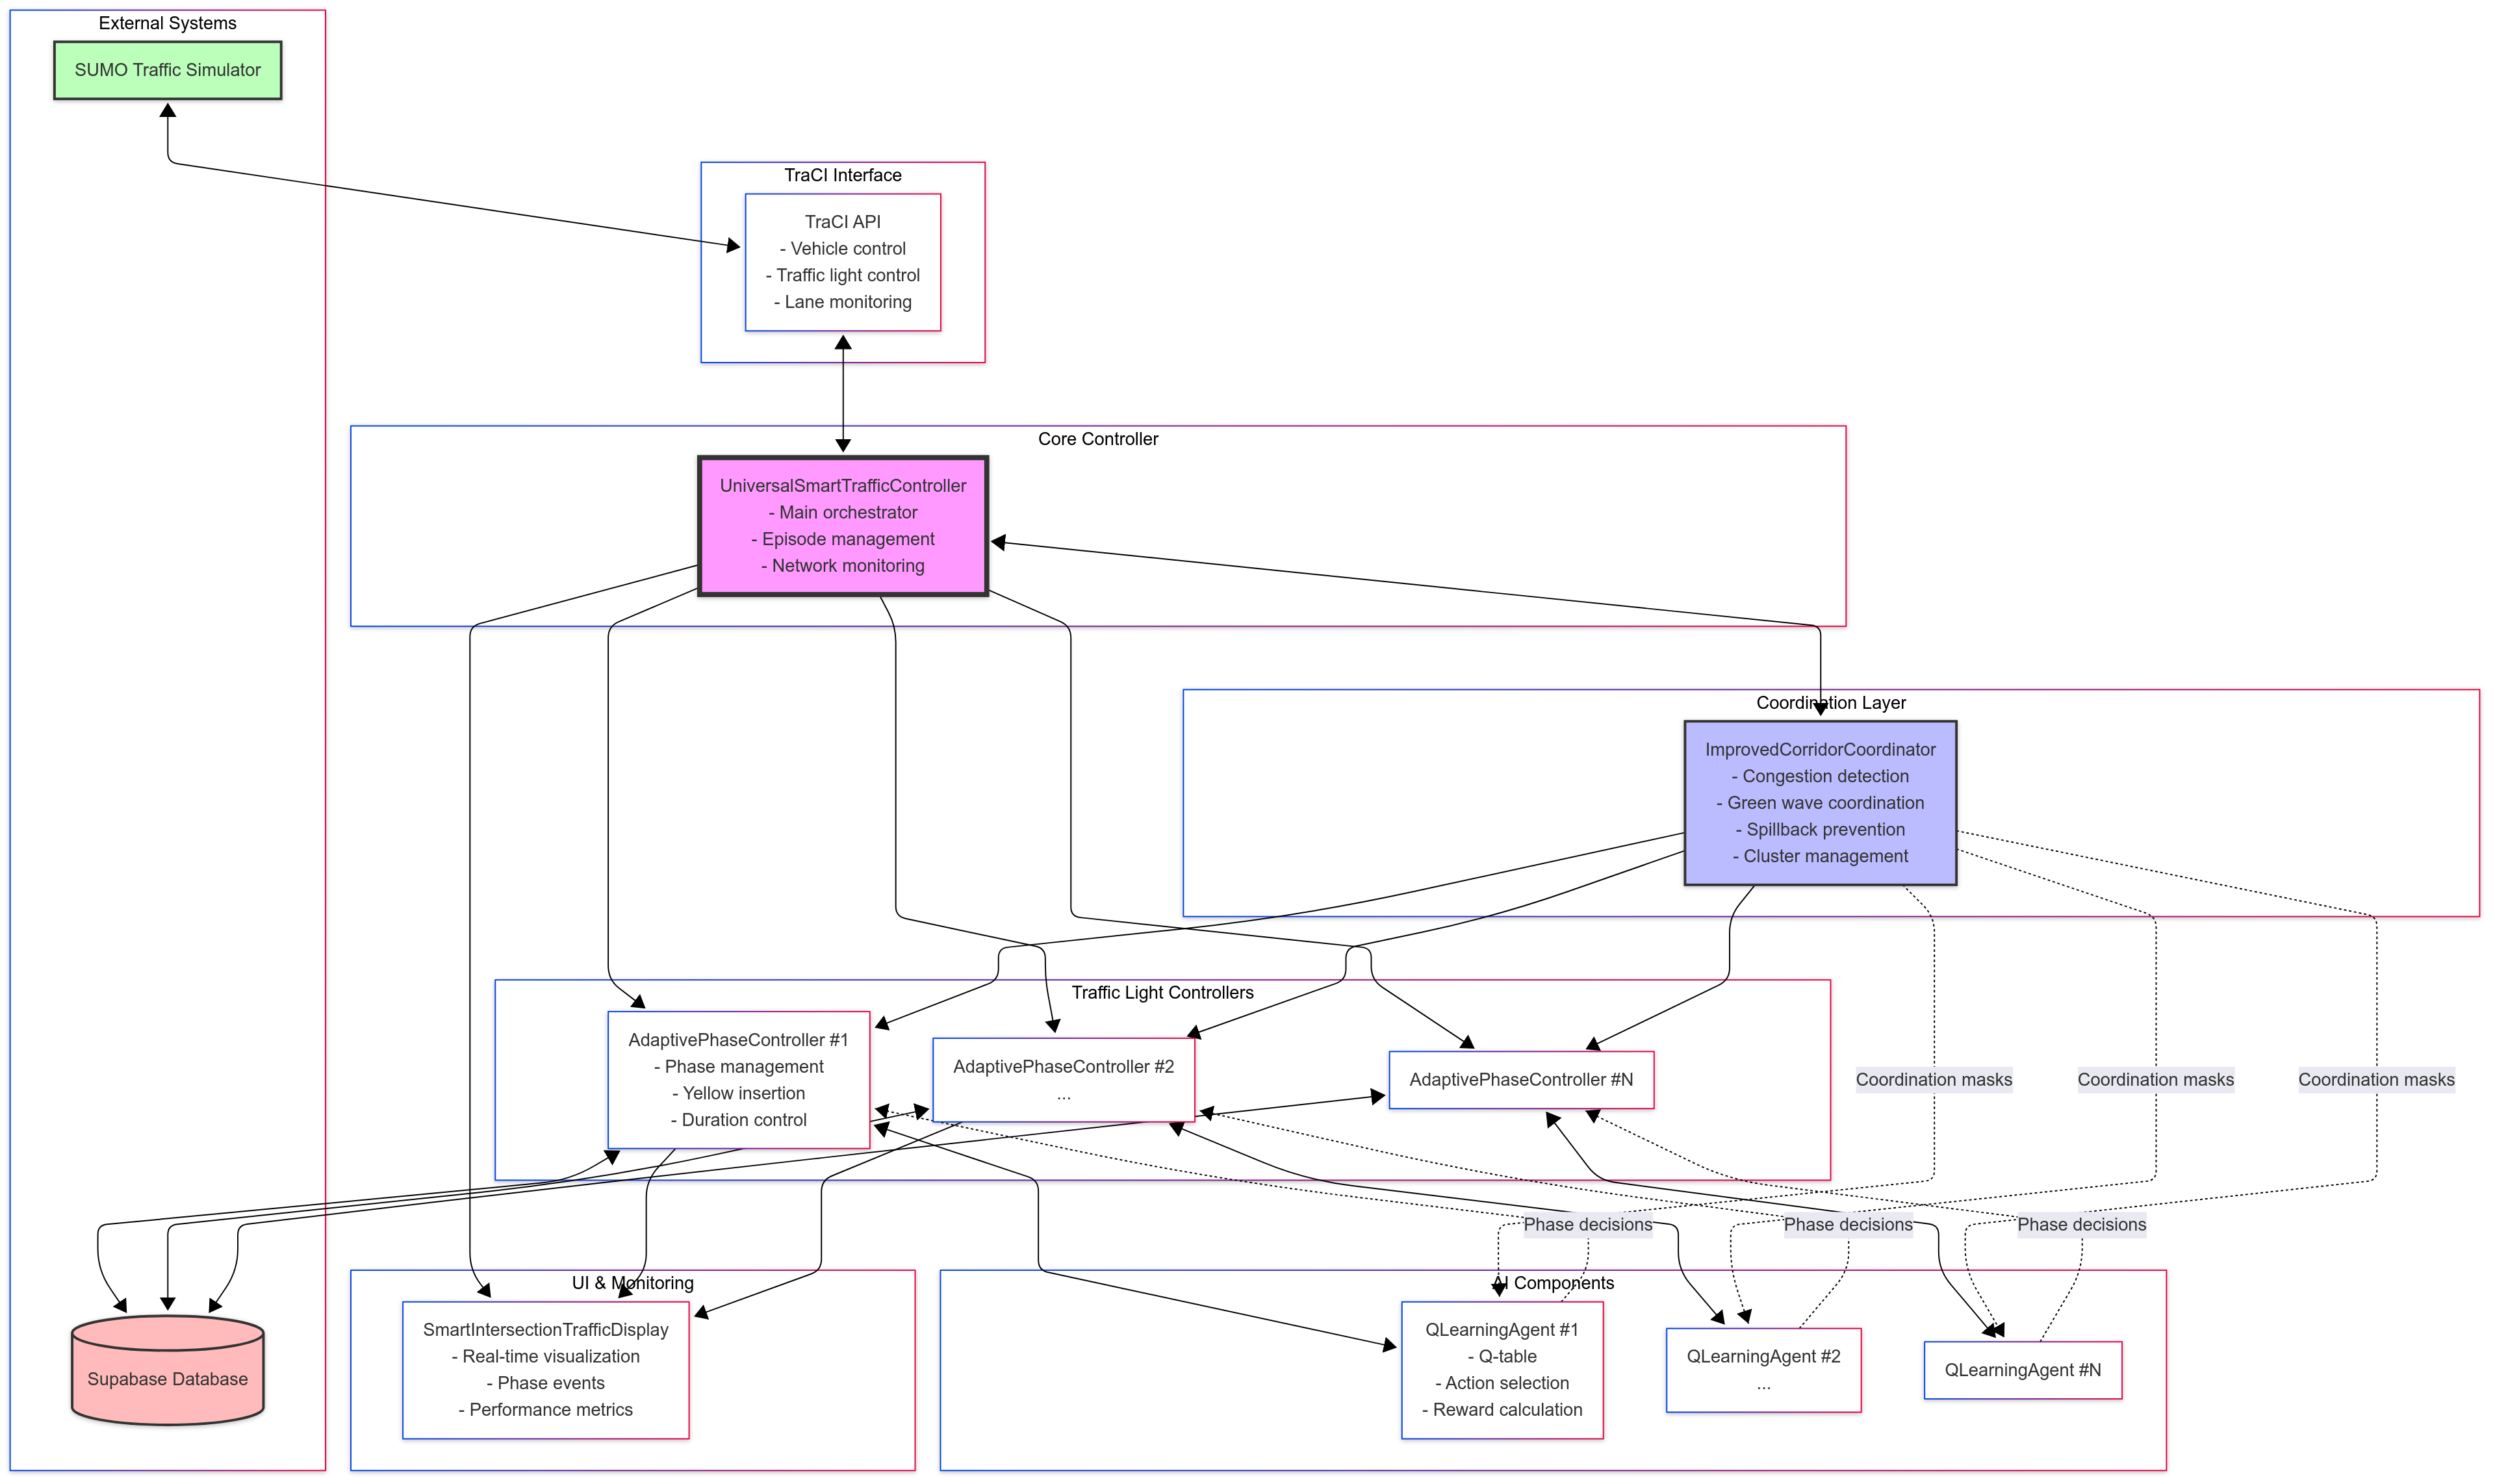
\includegraphics[width=1\linewidth]{Untitled diagram _ Mermaid Chart-2025-08-21-023904.png}

    
    \caption{Kiến trúc tổng thể hệ thống điều khiển đèn giao thông thông minh}
    \label{fig:system_architecture}
\end{figure}

Hệ thống bao gồm 4 tầng chính:

\textbf{Tầng mô phỏng (Simulation Layer):} SUMO đóng vai trò là môi trường mô phỏng giao thông vi mô (microscopic), cung cấp dữ liệu thời gian thực về trạng thái các phương tiện, làn đường và tín hiệu đèn. Đây là nền tảng để kiểm thử và đánh giá hiệu năng của các thuật toán điều khiển trong điều kiện giao thông đa dạng.

\textbf{Tầng giao tiếp (Interface Layer):} TraCI (Traffic Control Interface) đóng vai trò cầu nối hai chiều giữa SUMO và hệ thống điều khiển Python. TraCI cho phép đọc trạng thái mô phỏng thông qua subscription mechanism và gửi lệnh điều khiển đèn tín hiệu theo từng bước thời gian với các wrapper function đảm bảo an toàn.

\textbf{Tầng điều khiển (Control Layer):} Lõi của hệ thống với kiến trúc phân cấp: UniversalSmartTrafficController làm bộ điều khiển trung tâm, quản lý nhiều AdaptivePhaseController (mỗi APC phụ trách một nút giao). Mỗi APC tích hợp với EnhancedQLearningAgent để ra quyết định tối ưu. Đặc biệt, ImprovedCorridorCoordinator điều phối nhiều nút giao, phát hiện cụm tắc nghẽn và tạo green wave cho tuyến đường chính.

\textbf{Tầng lưu trữ (Storage Layer):} Hệ thống hybrid với hai thành phần: (1) Supabase cung cấp cơ sở dữ liệu đám mây để lưu trữ trạng thái APC, lịch sử điều chỉnh pha và nhật ký sự kiện với cơ chế batch write và retry logic; (2) Local storage lưu Q-table trong file pickle để đảm bảo hiệu suất truy xuất nhanh trong quá trình học. SmartIntersectionTrafficDisplay cung cấp giao diện giám sát real-time và phân tích metrics.
\subsection{Luồng dữ liệu}

Luồng dữ liệu trong hệ thống hoạt động theo chu trình closed-loop:

\begin{enumerate}
    \item \textbf{Thu thập dữ liệu:} TraCI đọc trạng thái giao thông từ SUMO, bao gồm số lượng xe, tốc độ trung bình, hàng chờ và thời gian chờ trên mỗi làn đường.
    
    \item \textbf{Xử lý và phân tích:} UniversalSmartTrafficController tổng hợp dữ liệu từ tất cả các làn đường, tính toán các chỉ số hiệu suất như mật độ, lưu lượng và mức độ tắc nghẽn.
    
    \item \textbf{Ra quyết định:} AdaptivePhaseController kết hợp với QLearningAgent để đưa ra quyết định chuyển pha hoặc điều chỉnh thời lượng dựa trên trạng thái hiện tại và kinh nghiệm học được.
    
    \item \textbf{Thực thi điều khiển:} Lệnh điều khiển được gửi ngược lại SUMO thông qua TraCI để thay đổi trạng thái đèn tín hiệu.
    
    \item \textbf{Lưu trữ và học:} Kết quả hành động và phần thưởng được lưu vào Supabase, cập nhật Q-table để cải thiện quyết định trong tương lai.
\end{enumerate}

\subsection{Các điểm tích hợp}

Hệ thống được thiết kế với nhiều điểm tích hợp linh hoạt:

\textbf{TraCI API:} Cung cấp hơn 100 hàm API để tương tác với SUMO, từ đọc thông tin cơ bản đến điều khiển phức tạp. Các subscription được sử dụng để tối ưu băng thông, chỉ lấy dữ liệu cần thiết.

\textbf{Supabase REST API:} Cho phép đồng bộ dữ liệu không đồng bộ với cơ sở dữ liệu đám mây, hỗ trợ batch insert để giảm độ trễ và tăng throughput.

\textbf{Corridor Coordinator Interface:} Module ImprovedCorridorCoordinator cung cấp khả năng điều phối nhiều nút giao, phát hiện cụm tắc nghẽn và tối ưu hóa luồng giao thông trên toàn mạng lưới.

\section{Các thành phần cốt lõi}

\subsection{Bộ điều khiển giao thông thông minh tổng quát}

UniversalSmartTrafficController là thành phần điều khiển cấp cao nhất, chịu trách nhiệm:

\begin{itemize}
    \item \textbf{Quản lý đa nút giao:} Khởi tạo và quản lý nhiều AdaptivePhaseController, mỗi bộ điều khiển phụ trách một nút giao thông độc lập.
    
    \item \textbf{Thu thập dữ liệu toàn cục:} Tổng hợp thông tin từ tất cả các làn đường trong mạng lưới thông qua lane subscription với TraCI.
    
    \item \textbf{Phân tích mạng lưới:} Xác định làn rẽ trái/phải, phát hiện tuyến đường chính (arterial), tính toán mức độ nghẽn cho từng khu vực.
    
    \item \textbf{Điều phối chiến lược:} Kích hoạt chế độ ưu tiên khẩn cấp, chế độ chống tắc nghẽn toàn cục, và điều phối green wave cho tuyến chính.
\end{itemize}

Controller duy trì các cấu trúc dữ liệu quan trọng như \texttt{lane\_to\_tl} (ánh xạ làn-đèn), \texttt{tl\_action\_sizes} (số pha mỗi đèn), và \texttt{intersection\_data} (dữ liệu thời gian thực).

\subsection{Bộ điều khiển pha thích nghi (APC)}

AdaptivePhaseController thực hiện điều khiển cấp nút giao với các chức năng:

\textbf{Điều chỉnh pha động:} Module \texttt{adjust\_phase\_duration()} tính toán thời lượng pha tối ưu dựa trên hàng chờ, thời gian chờ và mật độ giao thông. Công thức điều chỉnh:
\[
\Delta t = \alpha \cdot (R - R_{target})
\]
trong đó $R$ là phần thưởng hiện tại, $R_{target}$ là mục tiêu động, và $\alpha$ là hệ số học.

\textbf{Quản lý pha đèn vàng:} Hàm \texttt{insert\_yellow\_phase\_if\_needed()} tự động chèn pha vàng an toàn khi chuyển từ xanh sang đỏ, với thời lượng thích ứng theo tốc độ phương tiện và chiều dài hàng chờ.

\textbf{Xử lý rẽ trái bảo vệ:} Module \texttt{detect\_blocked\_left\_turn\_with\_conflict()} phát hiện làn rẽ trái bị chặn và kích hoạt pha bảo vệ riêng để giải phóng.

\textbf{Ưu tiên khẩn cấp:} Hệ thống hàng đợi ưu tiên \texttt{pending\_requests} quản lý các yêu cầu chuyển pha theo mức độ ưu tiên: emergency > critical\_starvation > heavy\_congestion > normal.

\subsection{Tác tử Q-learning cải tiến}

EnhancedQLearningAgent triển khai thuật toán học tăng cường với các cải tiến:

\textbf{Không gian trạng thái:} Vector 12 chiều mã hóa thông tin giao thông toàn diện:
\begin{itemize}
    \item Chỉ số hàng chờ (max, mean)
    \item Tốc độ phương tiện (min, mean)  
    \item Thời gian chờ (max, mean)
    \item Pha hiện tại và tổng số pha
    \item Hàng chờ làn rẽ trái/phải
\end{itemize}

\textbf{Cơ chế học thích ứng:} Tham số epsilon giảm dần theo \texttt{epsilon\_decay}, cân bằng giữa khám phá và khai thác. Optimistic initialization với giá trị 10.0 khuyến khích khám phá pha mới.

\textbf{Hàm thưởng đa mục tiêu:} Kết hợp nhiều yếu tố với trọng số thích ứng:
\[
R = 100 \cdot (-w_q \cdot Q + w_v \cdot V - w_w \cdot W - w_d \cdot D + bonus - penalty)
\]

\textbf{Tích hợp Coordinator:} Agent có thể nhận mask từ ImprovedCorridorCoordinator để hạn chế không gian hành động, đảm bảo phối hợp toàn cục.

\subsection{Lớp giao tiếp SUMO--TraCI}

TraCI Interface cung cấp abstraction layer cho việc tương tác với SUMO:

\textbf{Subscription Management:} Đăng ký theo dõi các biến quan trọng của làn đường và phương tiện, giảm overhead communication.

\textbf{Safe Phase Control:} Các wrapper function như \texttt{safe\_set\_phase()} và \texttt{\_safe\_phase\_index()} đảm bảo chỉ số pha luôn hợp lệ, tránh crash.

\textbf{Logic Cache:} Cache logic đèn tín hiệu với TTL 0.5s, giảm số lần query và tăng hiệu suất.

\section{Công nghệ sử dụng}

\subsection{Môi trường Python}

Hệ thống được phát triển với Python 3.8+, tận dụng các tính năng hiện đại:

\begin{itemize}
    \item \textbf{Async/Await:} Xử lý I/O không đồng bộ với Supabase
    \item \textbf{Type Hints:} Tăng độ tin cậy và khả năng bảo trì code
    \item \textbf{Dataclasses:} Quản lý cấu trúc dữ liệu phức tạp
    \item \textbf{Threading:} Chạy parallel cho database writer và display
\end{itemize}

\subsection{Mô phỏng giao thông SUMO}

SUMO (Simulation of Urban MObility) version 1.22.0 cung cấp:

\begin{itemize}
    \item \textbf{Microscopic simulation:} Mô phỏng từng phương tiện riêng lẻ
    \item \textbf{Network editor:} Công cụ NETEDIT để thiết kế mạng lưới
    \item \textbf{Demand generation:} Tạo luồng giao thông thực tế
    \item \textbf{Output analysis:} Xuất dữ liệu chi tiết để đánh giá
\end{itemize}

\subsection{Tích hợp API TraCI}

TraCI 1.22.0 cung cấp Python binding với các module chính:

\begin{itemize}
    \item \texttt{traci.trafficlight}: Điều khiển đèn tín hiệu
    \item \texttt{traci.lane}: Đọc thông tin làn đường
    \item \texttt{traci.vehicle}: Theo dõi phương tiện
    \item \texttt{traci.simulation}: Quản lý mô phỏng
\end{itemize}

\subsection{Cấu hình Supabase}

Supabase cung cấp cơ sở dữ liệu PostgreSQL được quản lý trên đám mây với khả năng real-time và REST API tự động. Hệ thống sử dụng 4 bảng chính với cấu trúc được tối ưu cho việc lưu trữ và truy vấn dữ liệu giao thông:

\subsubsection{Bảng apc\_states}

Bảng chính lưu trữ trạng thái đầy đủ của các bộ điều khiển APC (Adaptive Phase Controller):

\begin{figure}[H]
    \centering
    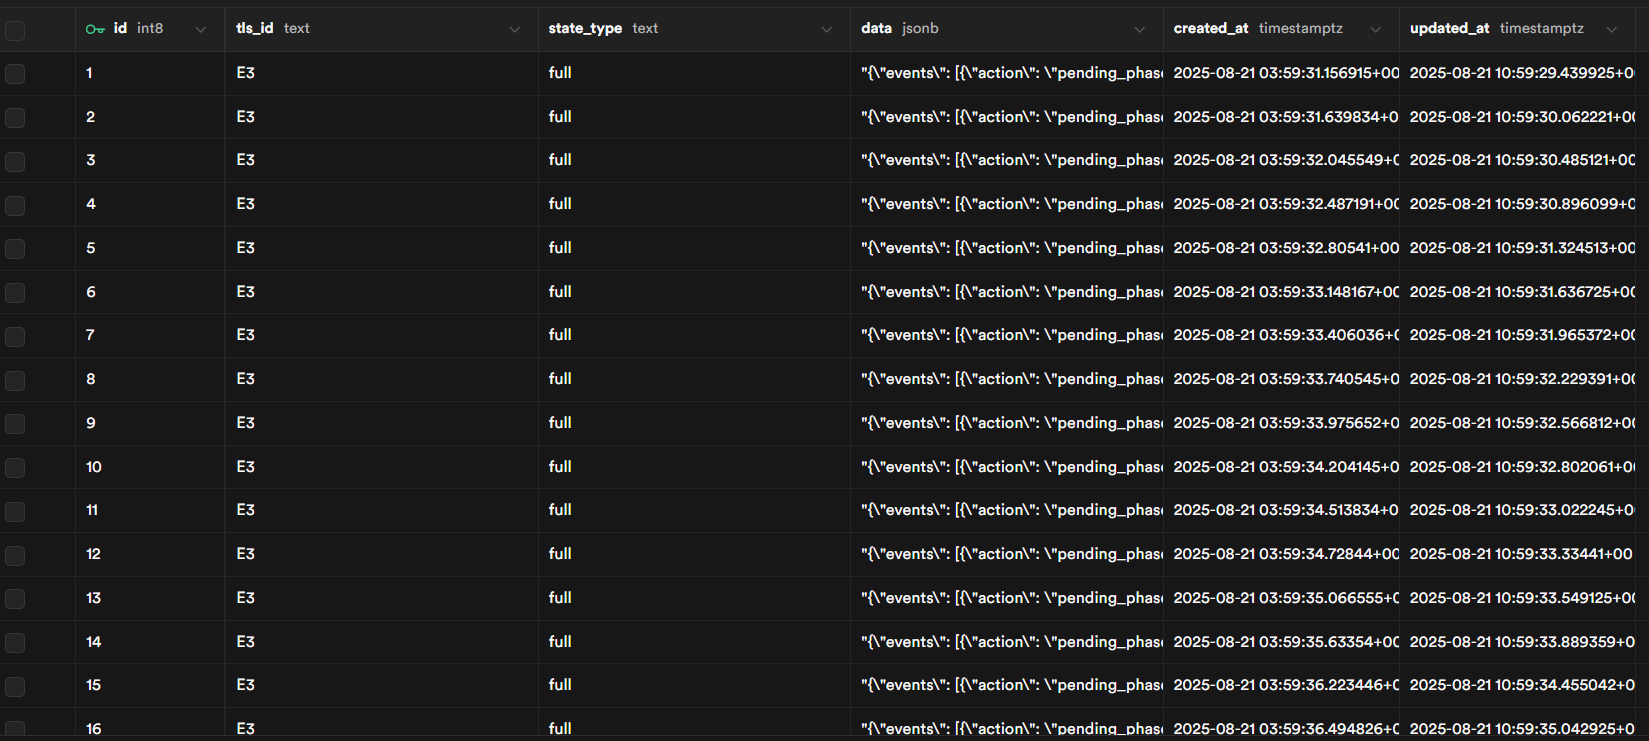
\includegraphics[width=1\linewidth]{tut.png}
    \caption{Dữ liệu mẫu trong bảng apc\_states}
    \label{fig:apc_states_data}
\end{figure}

Bảng \texttt{apc\_states} được thiết kế với cấu trúc linh hoạt để lưu trữ nhiều loại trạng thái khác nhau của hệ thống điều khiển:

\begin{lstlisting}[style=sql,caption={Định nghĩa cấu trúc bảng apc\_states}]
CREATE TABLE apc_states (
    id BIGSERIAL PRIMARY KEY,
    tls_id TEXT NOT NULL,           -- ID của nút giao thông
    state_type TEXT NOT NULL,       -- Loại trạng thái
    data JSONB NOT NULL,            -- Dữ liệu trạng thái
    created_at TIMESTAMPTZ DEFAULT NOW(),
    updated_at TIMESTAMPTZ DEFAULT NOW()
);

-- Tạo index để tối ưu truy vấn
CREATE INDEX idx_apc_states_tls_type 
    ON apc_states(tls_id, state_type);
CREATE INDEX idx_apc_states_data 
    ON apc_states USING gin(data);
\end{lstlisting}

Trường \texttt{state\_type} phân loại dữ liệu thành ba nhóm chính:

\begin{itemize}
    \item \textbf{\texttt{full}}: Snapshot toàn bộ trạng thái APC tại một thời điểm, bao gồm:
        \begin{itemize}
            \item Cấu hình các pha đèn (phase configurations)
            \item Hàng đợi sự kiện đang chờ xử lý
            \item Thông số điều khiển hiện tại
            \item Trạng thái của Q-learning agent
        \end{itemize}
    
    \item \textbf{\texttt{phase}}: Thông tin chi tiết về một pha đèn cụ thể:
        \begin{itemize}
            \item Thời lượng thực tế và cơ sở
            \item Danh sách làn đường được phục vụ
            \item Điều chỉnh thời gian ($\Delta t$)
        \end{itemize}
    
    \item \textbf{\texttt{event}}: Sự kiện điều khiển đơn lẻ:
        \begin{itemize}
            \item Chuyển pha khẩn cấp
            \item Kích hoạt rẽ trái bảo vệ
            \item Phát hiện tắc nghẽn
        \end{itemize}
\end{itemize}

Việc sử dụng JSONB cho trường \texttt{data} mang lại nhiều lợi ích:
- Linh hoạt trong việc mở rộng cấu trúc dữ liệu
- Hỗ trợ query và indexing hiệu quả với GIN index
- Dễ dàng tích hợp với Python thông qua JSON serialization

\subsubsection{Bảng phase\_records}

Lưu trữ lịch sử chi tiết về mọi điều chỉnh pha trong hệ thống:

\begin{table}[H]
\centering
\footnotesize
\begin{tabular}{|l|l|p{6cm}|}
\hline
\textbf{Cột} & \textbf{Kiểu dữ liệu} & \textbf{Mô tả} \\
\hline
\hline
\multicolumn{3}{|c|}{\textit{Thông tin cơ bản}} \\
\hline
id & BIGSERIAL & Khóa chính tự tăng \\
tls\_id & TEXT & ID của nút giao thông \\
phase\_idx & INTEGER & Chỉ số pha (0-11) \\
sim\_time & REAL & Thời điểm trong mô phỏng (giây) \\
\hline
\multicolumn{3}{|c|}{\textit{Thông số thời gian}} \\
\hline
duration & REAL & Thời lượng thực tế của pha (giây) \\
base\_duration & REAL & Thời lượng cơ sở theo cấu hình \\
delta\_t & REAL & Mức điều chỉnh sau làm mượt \\
raw\_delta\_t & REAL & Mức điều chỉnh ban đầu \\
extended\_time & REAL & Thời gian mở rộng thêm \\
\hline
\multicolumn{3}{|c|}{\textit{Thông tin điều khiển}} \\
\hline
state\_str & TEXT & Chuỗi trạng thái (vd: "GGrrGGrr") \\
event\_type & TEXT & Loại sự kiện kích hoạt điều chỉnh \\
weights & JSONB & Trọng số các yếu tố điều khiển \\
lanes & JSONB & Danh sách làn đường được phục vụ \\
\hline
\multicolumn{3}{|c|}{\textit{Đánh giá hiệu suất}} \\
\hline
reward & REAL & Phần thưởng từ RL agent \\
penalty & REAL & Hình phạt cho điều chỉnh quá mức \\
bonus & REAL & Điểm thưởng cho hiệu suất tốt \\
\hline
\multicolumn{3}{|c|}{\textit{Metadata}} \\
\hline
created\_at & TIMESTAMPTZ & Thời điểm tạo bản ghi \\
updated\_at & TIMESTAMPTZ & Thời điểm cập nhật cuối \\
\hline
\end{tabular}
\caption{Cấu trúc chi tiết bảng phase\_records với phân nhóm theo chức năng}
\label{tab:phase_records_detailed}
\end{table}

Bảng này đóng vai trò quan trọng trong việc:
\begin{itemize}
    \item Theo dõi lịch sử điều chỉnh để phân tích hiệu suất
    \item Cung cấp dữ liệu huấn luyện cho Q-learning agent
    \item Phát hiện các pattern giao thông lặp lại
    \item Debug và tối ưu hóa thuật toán điều khiển
\end{itemize}

\subsubsection{Bảng simulation\_events}

Ghi nhận mọi sự kiện trong quá trình mô phỏng:

\begin{figure}[H]
    \centering
    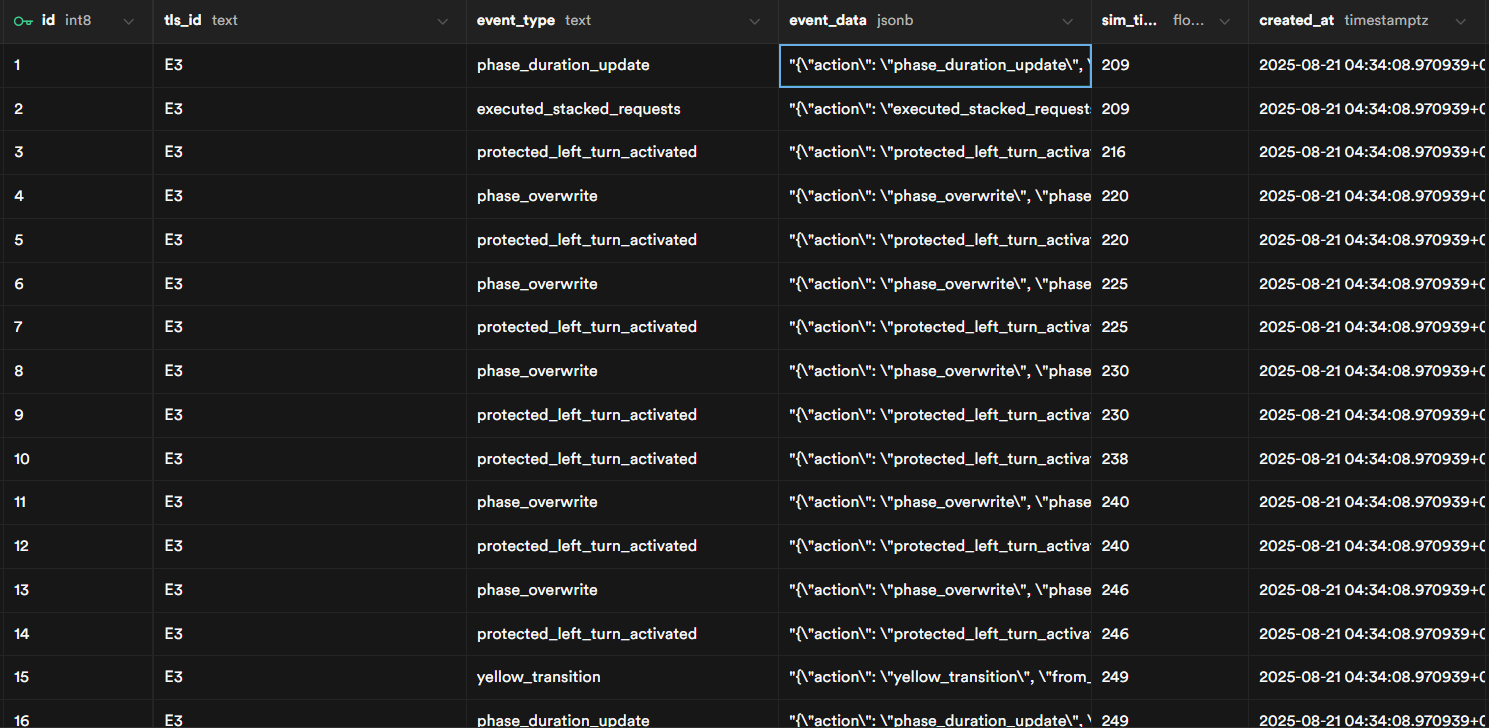
\includegraphics[width=1\linewidth]{TUTU.png}
    \caption{Dữ liệu thực tế từ bảng simulation\_events}
    \label{fig:simulation_events_data}
\end{figure}

Bảng \texttt{simulation\_events} (Hình \ref{fig:simulation_events_data}) lưu trữ lịch sử chi tiết các sự kiện điều khiển đèn giao thông với cấu trúc:

\begin{itemize}
    \item \texttt{id}: Khóa chính tự tăng (int8)
    \item \texttt{tls\_id}: ID của đèn giao thông (text) - trong ví dụ là "E3"
    \item \texttt{event\_type}: Loại sự kiện điều khiển (text)
    \item \texttt{event\_date}: Dữ liệu JSON chứa chi tiết sự kiện (jsonb)
    \item \texttt{sim\_time}: Thời điểm trong mô phỏng (float)
    \item \texttt{created\_at}: Thời điểm tạo bản ghi (timestamptz)
\end{itemize}

Ví dụ cấu trúc dữ liệu JSON trong cột \texttt{event\_date}:

\begin{lstlisting}[style=json,caption={Cấu trúc JSON của sự kiện phase\_duration\_update}]
{
    "action": "phase_duration_update",
    "phase": 209
}
\end{lstlisting}

\begin{lstlisting}[style=json,caption={Cấu trúc JSON của sự kiện phase\_overwrite}]
{
    "action": "phase_overwrite", 
    "phase": 220
}
\end{lstlisting}

Các loại sự kiện chính được ghi nhận trong hệ thống:
\begin{itemize}
    \item \texttt{phase\_duration\_update}: Cập nhật thời lượng pha đèn động
    \item \texttt{executed\_stacked\_requests}: Thực thi các yêu cầu đã được xếp hàng đợi
    \item \texttt{protected\_left\_turn\_activated}: Kích hoạt pha rẽ trái được bảo vệ
    \item \texttt{phase\_overwrite}: Ghi đè pha hiện tại với cấu hình mới
    \item \texttt{yellow\_transition}: Chuyển sang pha đèn vàng an toàn
\end{itemize}

Dữ liệu trong bảng cho thấy hệ thống liên tục điều chỉnh hoạt động, với các sự kiện được ghi nhận theo thời gian thực. Đặc biệt, sự kiện \texttt{protected\_left\_turn\_activated} xuất hiện nhiều lần (8/16 bản ghi), cho thấy hệ thống thường xuyên phải xử lý tình huống rẽ trái phức tạp tại nút giao này.


\subsubsection{Tối ưu hiệu suất database}

Hệ thống áp dụng nhiều kỹ thuật tối ưu:

\textbf{Indexing chiến lược:} Tạo composite index cho các truy vấn thường xuyên:
\begin{lstlisting}[style=sql]
CREATE INDEX idx_apc_states_tls_type 
    ON apc_states(tls_id, state_type);
CREATE INDEX idx_phase_records_phase_idx 
    ON phase_records(tls_id, phase_idx);
\end{lstlisting}

\textbf{JSONB cho flexibility:} Sử dụng JSONB thay vì JSON thuần để có khả năng index và query hiệu quả với GIN index.

\textbf{Row Level Security (RLS):} Bảo mật ở cấp độ row với policy:
\begin{lstlisting}[style=sql]
ALTER TABLE apc_states ENABLE ROW LEVEL SECURITY;
CREATE POLICY "Enable all operations for authenticated users" 
    ON apc_states
    FOR ALL USING (auth.role() = 'authenticated');
\end{lstlisting}

\textbf{Batch operations:} Module PatchedAsyncSupabaseWriter thực hiện batch insert với kích thước tối đa 100 records và interval 60 giây, giảm số lượng round-trip đến database.

\subsubsection{Chiến lược đồng bộ dữ liệu}

Hệ thống sử dụng mô hình write-behind cache:

\begin{enumerate}
    \item \textbf{Buffer cục bộ:} Dữ liệu được tích lũy trong \texttt{\_pending\_db\_ops} với giới hạn \texttt{MAX\_PENDING\_DB\_OPS = 1000}
    
    \item \textbf{Flush định kỳ:} AsyncSupabaseWriter flush dữ liệu mỗi 60 giây hoặc khi buffer đầy
    
    \item \textbf{Retry logic:} Exponential backoff với max 6 lần retry cho mỗi batch
    
    \item \textbf{Graceful degradation:} Nếu Supabase không khả dụng, hệ thống vẫn hoạt động với local cache
\end{enumerate}

Thiết kế này đảm bảo hệ thống có thể xử lý hàng triệu events mỗi giờ mà không ảnh hưởng đến hiệu suất real-time của điều khiển giao thông.

Hệ thống sử dụng các thư viện Python sau:

\begin{itemize}
    \item \textbf{NumPy 1.24+:} Tính toán ma trận và vector hiệu suất cao
    \item \textbf{Pandas 2.0+:} Xử lý và phân tích dữ liệu dạng bảng
    \item \textbf{Matplotlib 3.7+:} Trực quan hóa kết quả mô phỏng
    \item \textbf{Supabase-py 2.4+:} Client SDK cho Supabase
    \item \textbf{Threading, Queue:} Xử lý đa luồng và hàng đợi
    \item \textbf{Pickle:} Serialize/deserialize Q-table
\end{itemize}

Kiến trúc module này đảm bảo hệ thống có khả năng mở rộng, dễ bảo trì và hiệu suất cao trong việc điều khiển giao thông thông minh.

% =========================
% CHƯƠNG 5
% =========================
% =========================
% CHƯƠNG 5
% =========================
\chapter{Điều khiển pha thích nghi (APC)}

\section{Nguyên lý thiết kế và kiến trúc}

Bộ điều khiển pha thích nghi (Adaptive Phase Controller - APC) được thiết kế theo nguyên lý điều khiển phân tán với khả năng tự quyết định cục bộ cho từng nút giao thông. Kiến trúc này cho phép mỗi nút giao hoạt động độc lập trong khi vẫn có thể phối hợp với các nút lân cận thông qua cơ chế trao đổi thông tin. APC kết hợp giữa điều khiển dựa trên luật (rule-based control) để đảm bảo an toàn và điều khiển thích ứng (adaptive control) để tối ưu hiệu suất.

\begin{figure}[H]
    \centering
    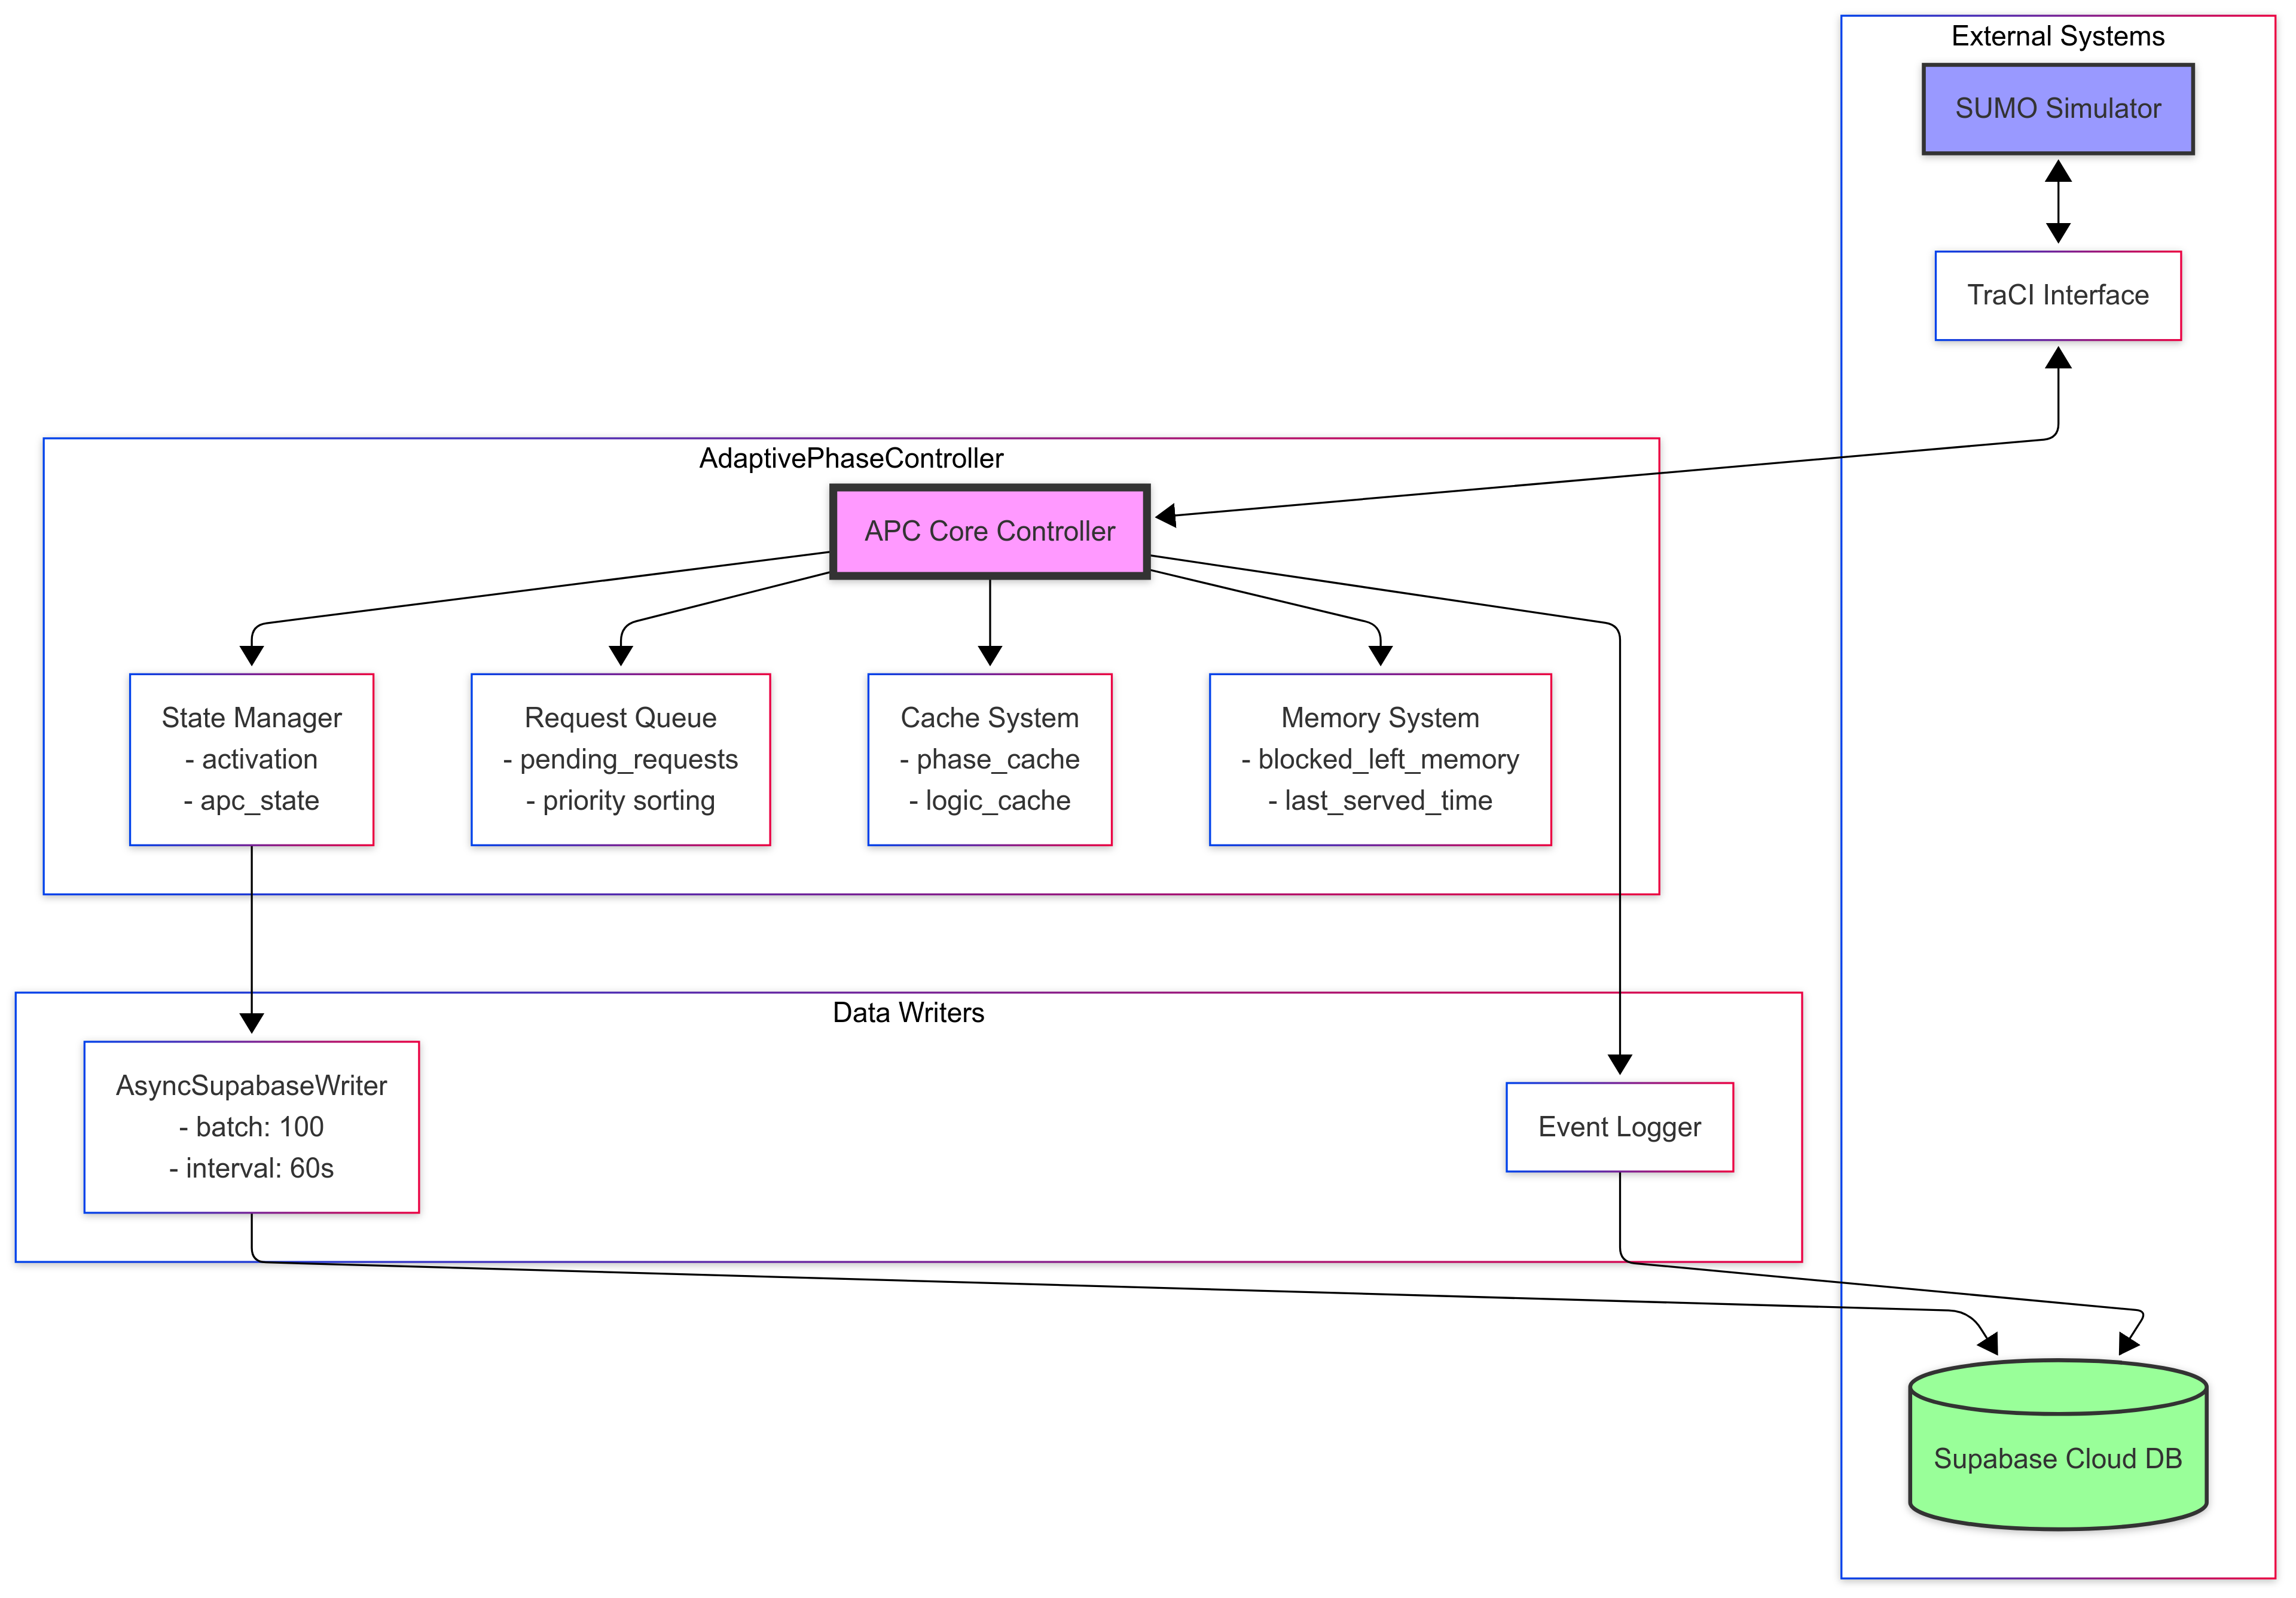
\includegraphics[width=0.9\textwidth]{Untitled diagram _ Mermaid Chart-2025-08-21-074754.png}
    \caption{Kiến trúc tổng thể của bộ điều khiển APC với các thành phần chính và luồng dữ liệu}
    \label{fig:apc_architecture}
\end{figure}

\subsection{Khởi tạo và cấu hình hệ thống}

Quá trình khởi tạo APC được thực hiện qua constructor với các tham số quan trọng:

\begin{lstlisting}[style=py, caption={Khởi tạo AdaptivePhaseController}]
def __init__(self, lane_ids, tls_id, alpha=1.0, 
             min_green=30, max_green=80,
             r_base=0.5, r_adjust=0.1, 
             severe_congestion_threshold=0.8,
             large_delta_t=20):
    self.lane_ids = lane_ids
    self.tls_id = tls_id
    # Đăng ký subscription với TraCI
    for lid in self.lane_ids:
        traci.lane.subscribe(lid, [
            traci.constants.LAST_STEP_VEHICLE_HALTING_NUMBER,
            traci.constants.LAST_STEP_MEAN_SPEED,
            traci.constants.LAST_STEP_VEHICLE_NUMBER,
            traci.constants.LAST_STEP_VEHICLE_ID_LIST,
        ])
\end{lstlisting}

\textbf{Quá trình khởi tạo bao gồm các bước chính:}

\begin{enumerate}
    \item \textbf{Thiết lập subscription với TraCI:} Hệ thống đăng ký theo dõi các metrics quan trọng cho từng làn đường được quản lý, bao gồm số lượng xe dừng, tốc độ trung bình, tổng số xe và danh sách ID phương tiện. Cơ chế subscription giúp tối ưu băng thông bằng cách chỉ nhận dữ liệu cần thiết.
    
    \item \textbf{Khởi tạo cấu trúc dữ liệu:} Các container quan trọng được khởi tạo:
    \begin{itemize}
        \item \texttt{apc\_state}: Dictionary lưu trữ trạng thái toàn cục với events queue (maxlen=5000) và danh sách phases
        \item \texttt{pending\_requests}: Hàng đợi yêu cầu chuyển pha với cơ chế ưu tiên
        \item \texttt{phase\_cache}: Cache thông tin pha với TTL 30 giây để giảm truy vấn database
        \item \texttt{blocked\_left\_memory}: Dictionary theo dõi lịch sử làn rẽ trái bị chặn
    \end{itemize}
    
    \item \textbf{Kết nối database:} Khởi tạo \texttt{PatchedAsyncSupabaseWriter} với interval 60 giây và batch size 100 records để đồng bộ dữ liệu không đồng bộ lên cloud.
    
    \item \textbf{Tải trạng thái từ Supabase:} Phương thức \texttt{\_load\_apc\_state\_supabase()} được gọi để khôi phục trạng thái từ lần chạy trước, đảm bảo tính liên tục của hệ thống.
    
    \item \textbf{Đồng bộ pha với SUMO:} \texttt{preload\_phases\_from\_sumo()} đảm bảo tất cả các pha trong logic đèn được ghi nhận và có base duration phù hợp.
\end{enumerate}
\begin{figure}[H]
    \centering
    \begin{subfigure}[b]{0.65\textwidth}
        \centering
        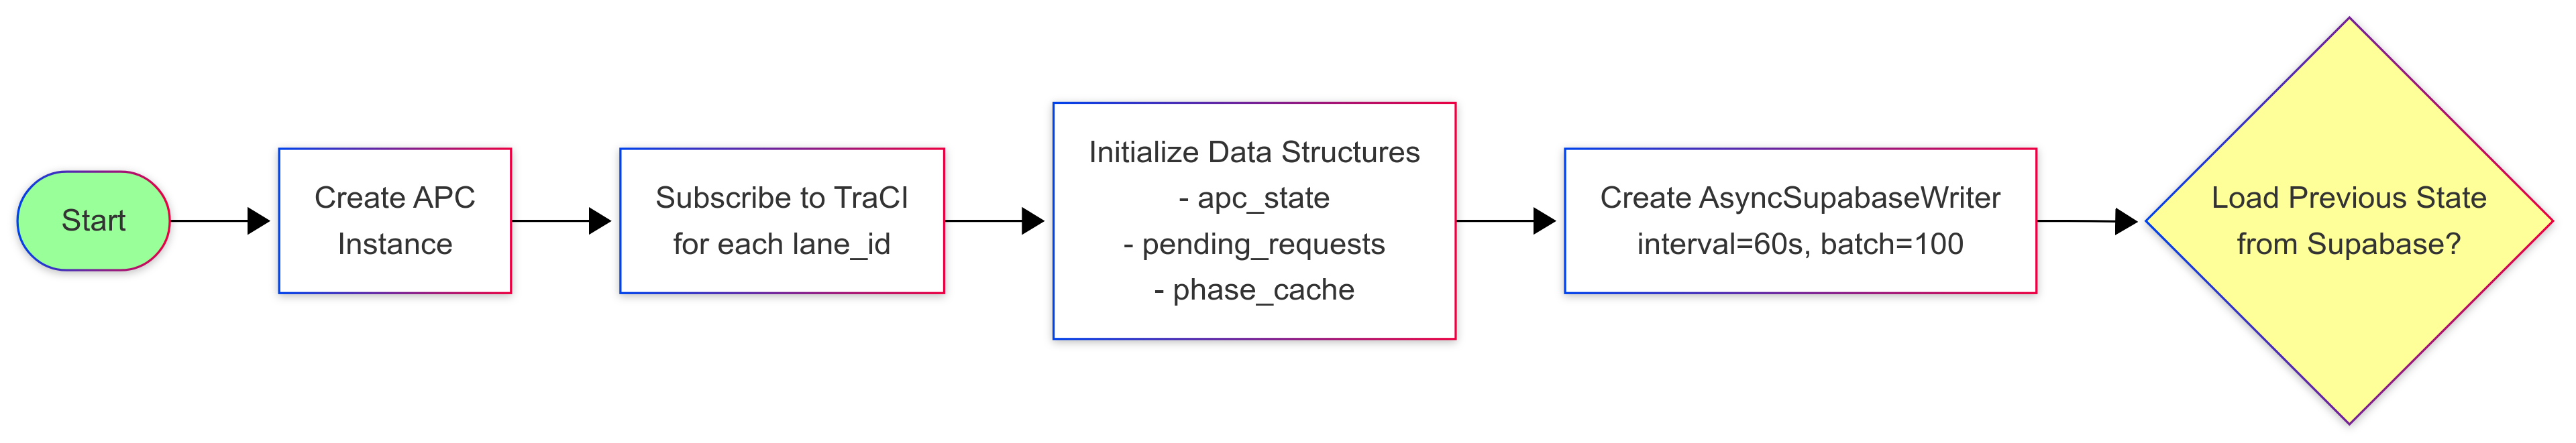
\includegraphics[width=\textwidth]{Untitled diagram _ Mermaid Chart-2025-08-21-084042.png}
        \caption{Khởi tạo và thiết lập}
    \end{subfigure}
    \hfill
    \begin{subfigure}[b]{0.65\textwidth}
        \centering
        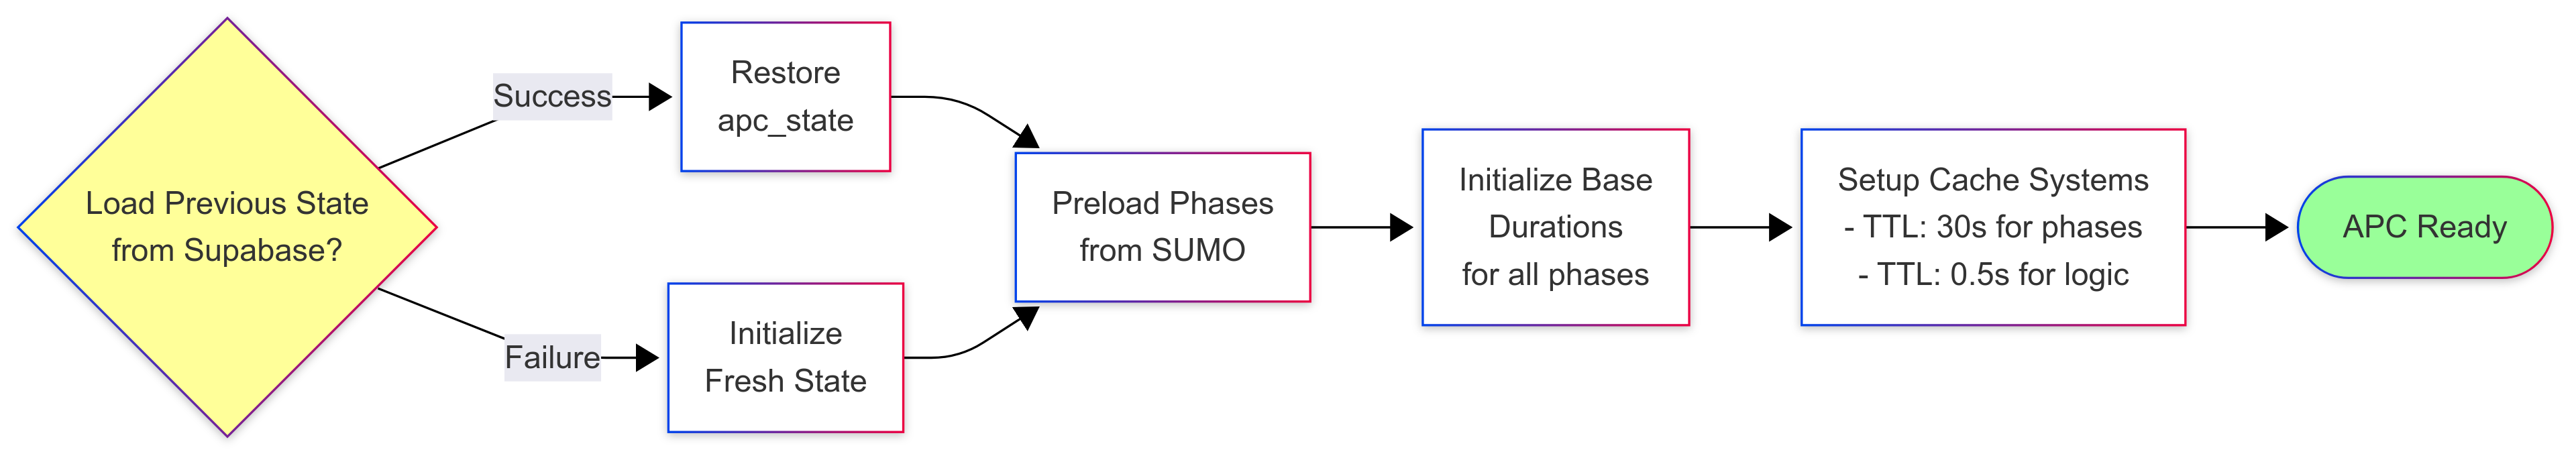
\includegraphics[width=\textwidth]{Untitled diagram _ Mermaid Chart-2025-08-21-084132.png}
        \caption{Khôi phục trạng thái và hoàn tất}
    \end{subfigure}
    \caption{Quy trình khởi tạo AdaptivePhaseController. \newline \textbf{Lưu ý:} Đã tăng kích thước hình để dễ quan sát hơn.}
    \label{fig:apc_init_flow}
\end{figure}
\subsection{Cấu trúc dữ liệu và tham số điều khiển}

APC sử dụng hệ thống tham số phân cấp để điều chỉnh hành vi:

\subsubsection{Tham số thời gian}
\begin{itemize}
    \item \texttt{min\_green} (mặc định 30s): Thời gian tối thiểu cho mỗi pha xanh, đảm bảo an toàn và công bằng
    \item \texttt{max\_green} (mặc định 80s): Giới hạn trên để tránh monopoly một hướng
    \item \texttt{cycle\_length} (mặc định 90s): Chu kỳ tham chiếu cho điều phối corridor
    \item \texttt{low\_demand\_extend\_cap} (4s): Giới hạn mở rộng khi nhu cầu thấp
\end{itemize}

\subsubsection{Tham số điều khiển thích ứng}
\begin{itemize}
    \item \texttt{alpha} (1.0): Hệ số học trong công thức điều chỉnh $\Delta t = \alpha(R - R_{target})$
    \item \texttt{r\_base} (0.5): Giá trị reward cơ sở cho thuật toán học
    \item \texttt{r\_adjust} (0.1): Hệ số điều chỉnh R\_target động
    \item \texttt{weights} (vector 4D): Trọng số cho [density, speed, wait, queue] trong hàm reward
\end{itemize}

\subsubsection{Ngưỡng phát hiện sự kiện}
\begin{itemize}
    \item \texttt{severe\_congestion\_threshold} (0.8): Tỷ lệ queue/capacity kích hoạt chế độ khẩn cấp
    \item \texttt{protected\_left\_min\_queue} (5): Số xe tối thiểu để kích hoạt rẽ trái bảo vệ
    \item \texttt{min\_starve\_queue} (2): Ngưỡng phát hiện starvation
    \item \texttt{hysteresis\_margin} (0.10): Yêu cầu cải thiện 10\% để chuyển pha
\end{itemize}
\begin{figure}[H]
    \centering
    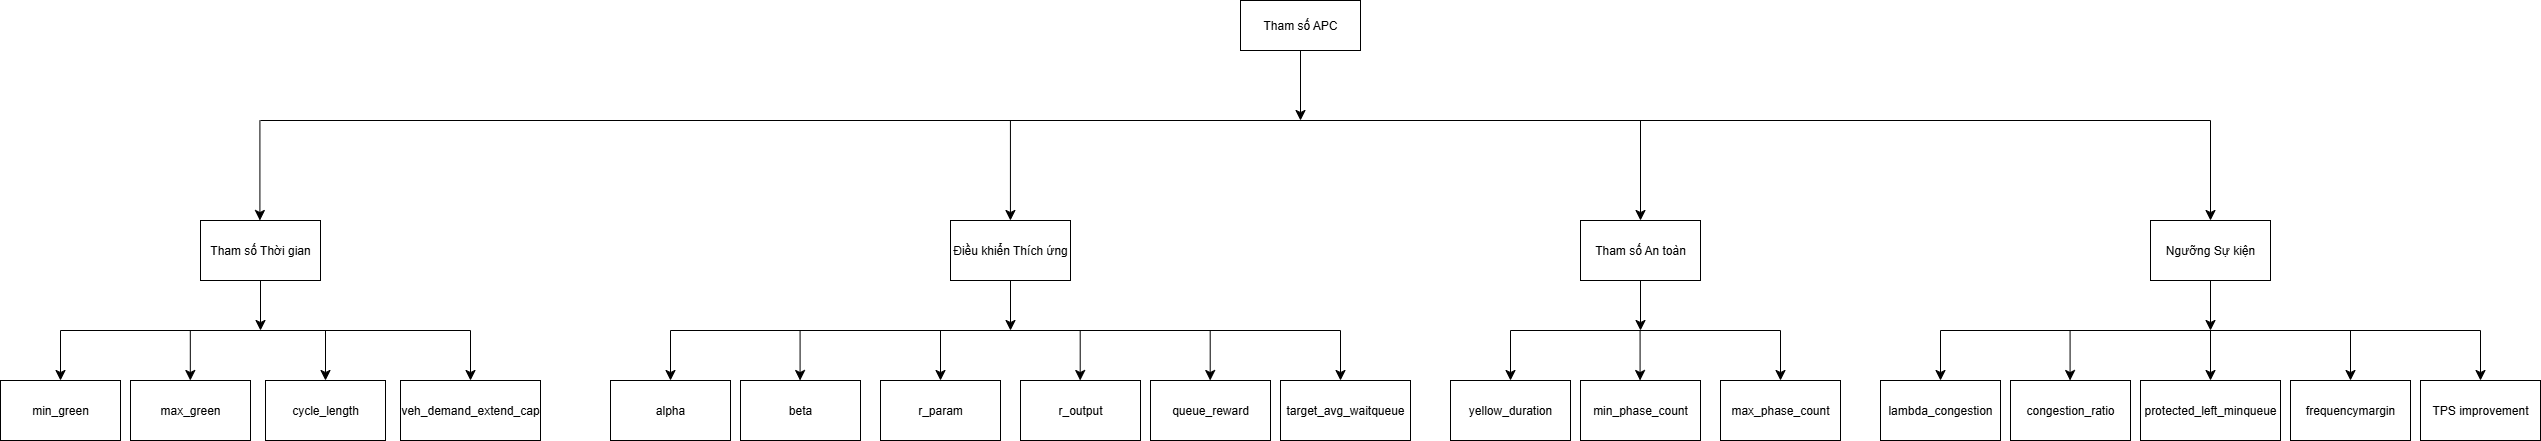
\includegraphics[width=1.1\textwidth]{Untitled Diagram.drawio (8).png}
    \caption{Phân cấp tham số điều khiển trong APC}
    \label{fig:parameter_hierarchy}
\end{figure}
\subsubsection{Cấu trúc dữ liệu chính}

\textbf{Activation State:} Dictionary theo dõi pha đang hoạt động:
\begin{lstlisting}[style=py]
self.activation = {
    "phase_idx": None,        # Chi so pha hien tai
    "start_time": 0.0,        # Thoi diem bat dau
    "base_duration": None,    # Thoi luong co so
    "desired_total": None     # Thoi luong mong muon
}
\end{lstlisting}

\textbf{Pending Requests Queue:} Danh sách các yêu cầu chuyển pha được sắp xếp theo priority và timestamp:
\begin{lstlisting}[style=py]
request = {
    "phase_idx": int,         # Pha muc tieu
    "priority": int,          # Muc uu tien (1-11)
    "priority_type": str,     # Loai: emergency, starvation...
    "extension_duration": float,  # Thoi luong yeu cau
    "timestamp": float        # Thoi diem tao yeu cau
}
\end{lstlisting}
\begin{figure}[H]
    \centering
    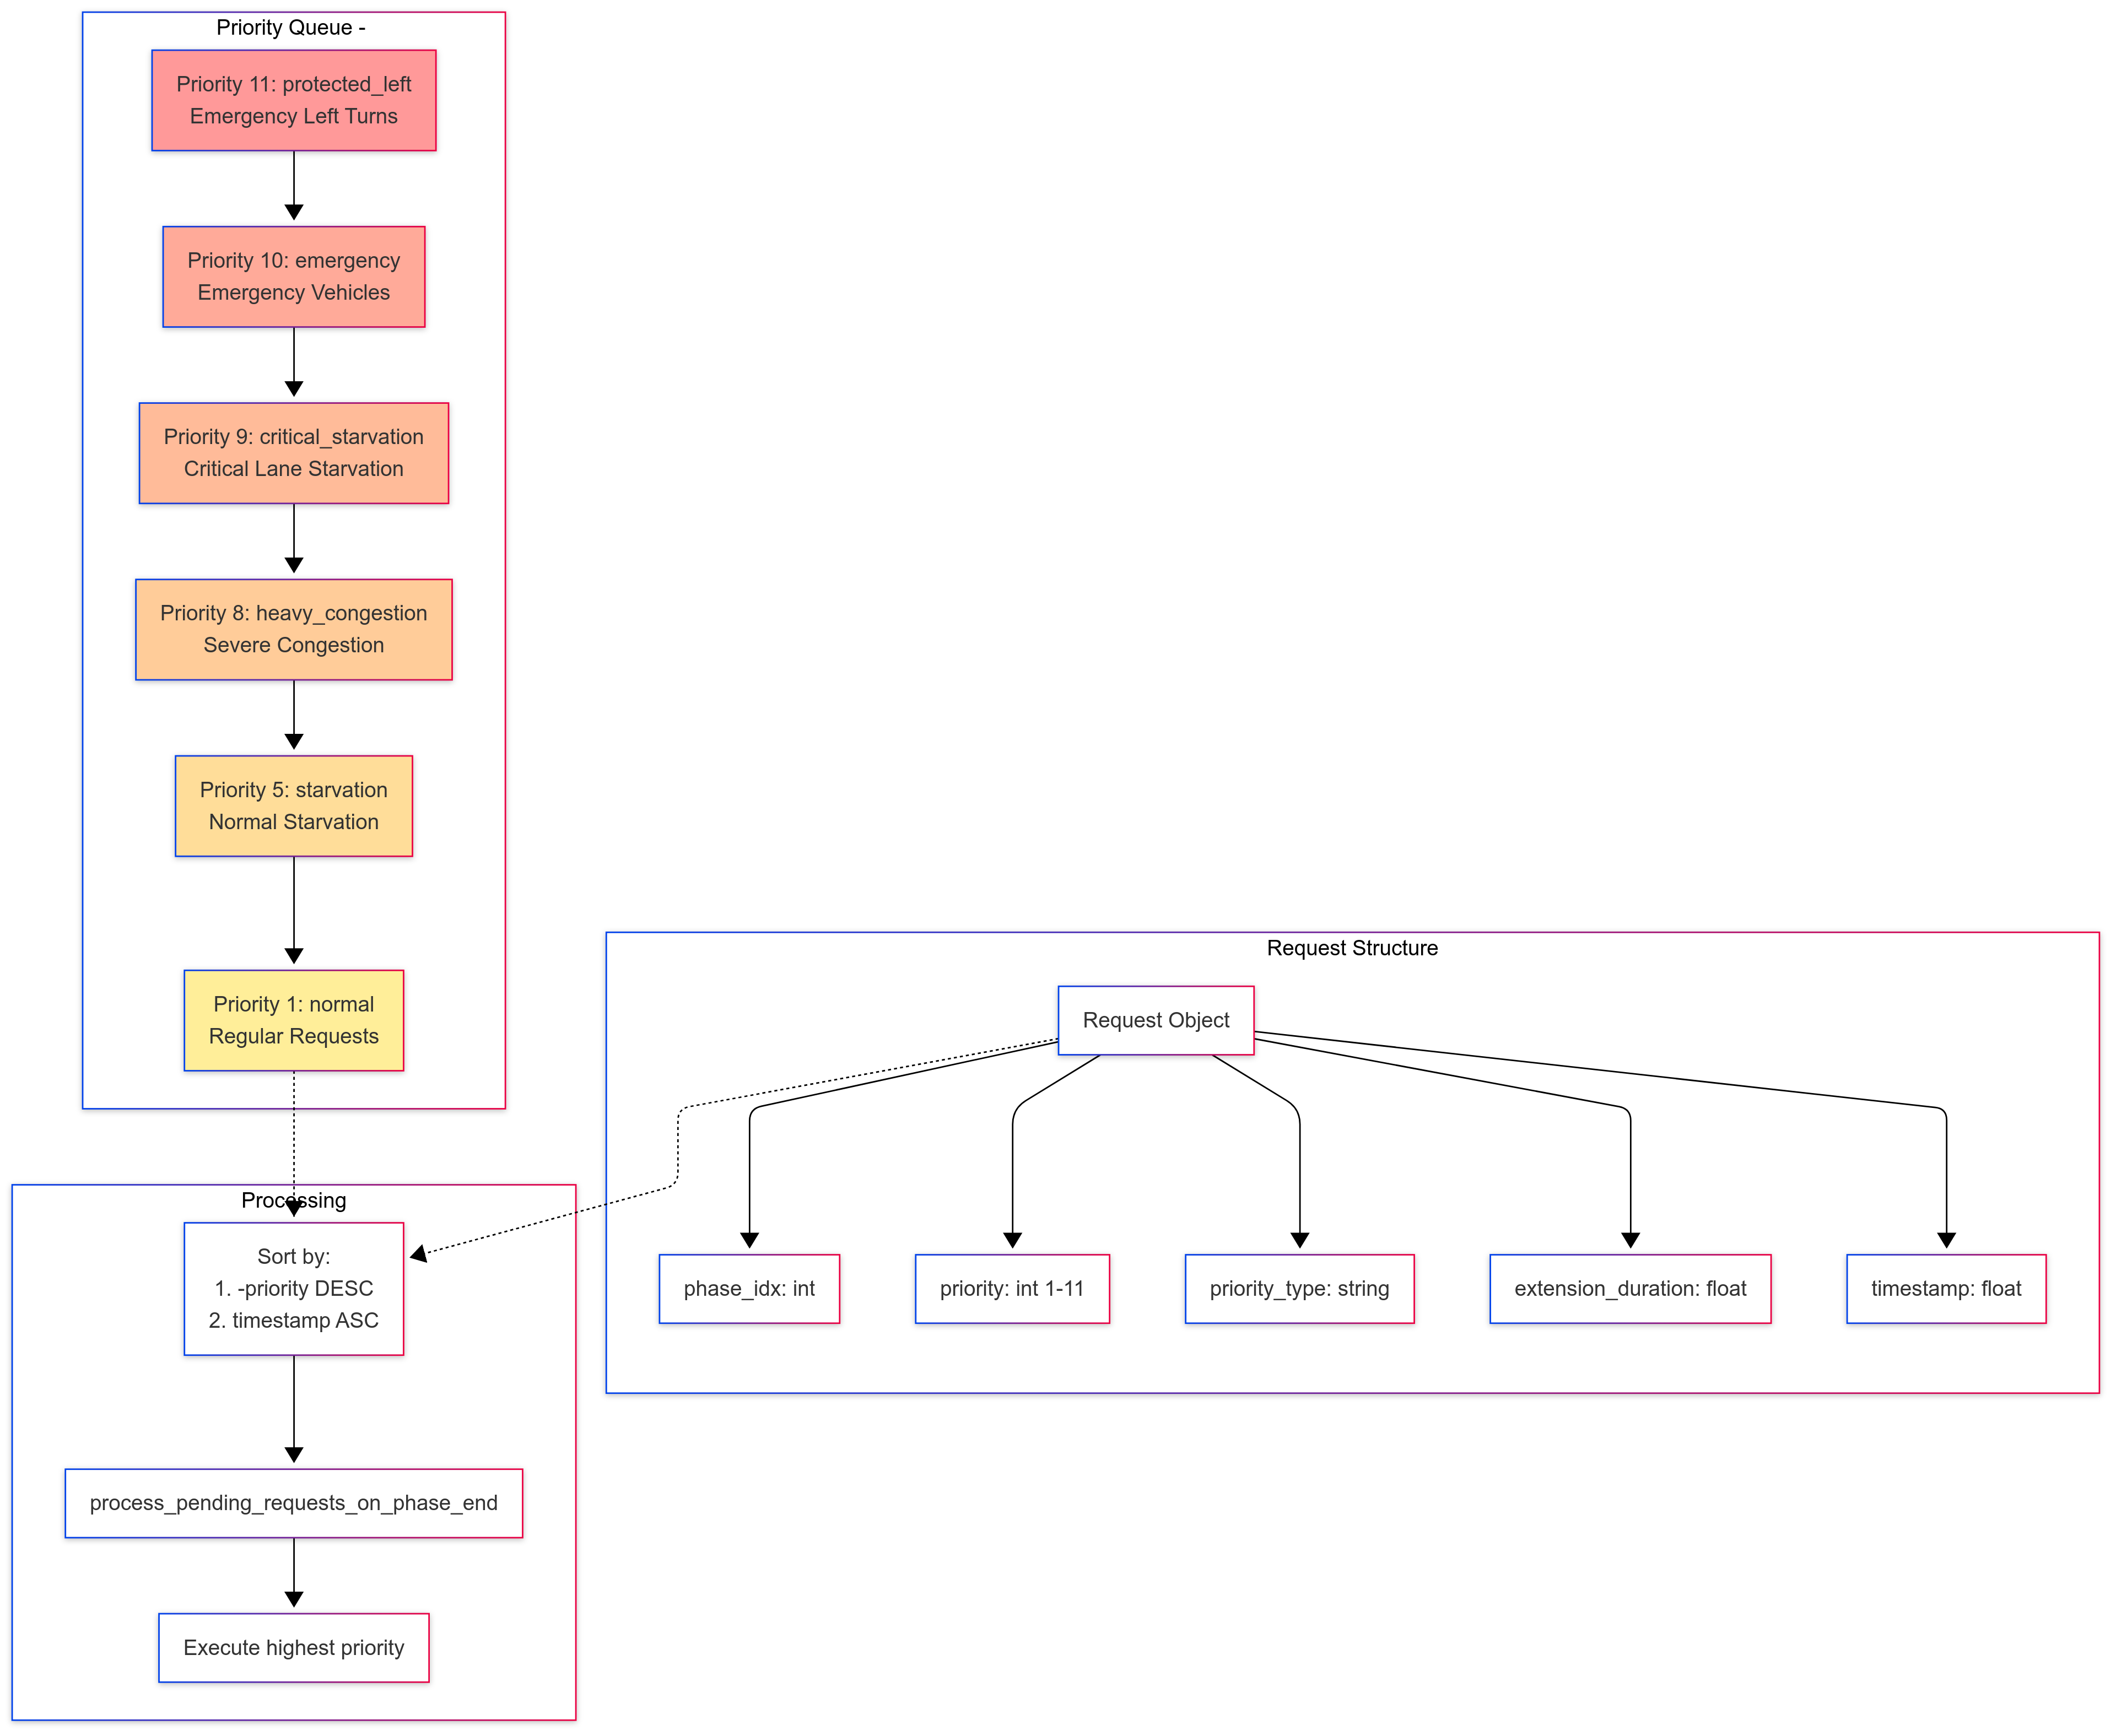
\includegraphics[width=0.75\textwidth]{Untitled diagram _ Mermaid Chart-2025-08-22-023041.png}
    \caption{Cấu trúc hàng đợi yêu cầu với mức độ ưu tiên}
    \label{fig:priority_queue}
\end{figure}
\subsection{Tích hợp với TraCI và SUMO}

Việc tích hợp với SUMO thông qua TraCI được thực hiện qua nhiều lớp abstraction:

\subsubsection{Subscription Mechanism}
APC sử dụng TraCI subscription để nhận dữ liệu real-time hiệu quả:

\begin{lstlisting}[style=py, caption={Xử lý subscription results}]
def get_lane_stats(self, lane_id):
    res = traci.lane.getSubscriptionResults(lane_id) or {}
    q = float(res.get(
        traci.constants.LAST_STEP_VEHICLE_HALTING_NUMBER,
        traci.lane.getLastStepHaltingNumber(lane_id)
    ))
    v = float(res.get(
        traci.constants.LAST_STEP_MEAN_SPEED,
        traci.lane.getLastStepMeanSpeed(lane_id)
    ))
    return q, w, v, dens
\end{lstlisting}

\subsubsection{Logic Cache System}
Để giảm overhead communication, APC implement cache cho traffic light logic:

\begin{lstlisting}[style=py, caption={Cơ chế cache logic}]
def _get_logic(self):
    now = traci.simulation.getTime()
    if self._logic_cache is None or \
       now - self._logic_cache_at > self._logic_cache_ttl:
        self._logic_cache = get_current_logic(self.tls_id)
        self._logic_cache_at = now
    return self._logic_cache
\end{lstlisting}

Cache có TTL 0.5 giây và được invalidate khi có thay đổi cấu trúc pha. Hệ thống còn hỗ trợ shared cache ở controller level để tối ưu cho nhiều APC instances.

\subsubsection{Safe Control Wrappers}
Mọi lệnh điều khiển được wrap trong các hàm an toàn:

\begin{lstlisting}[style=py, caption={Safe phase control}]
def _apply_phase(self, phase_idx, duration):
    # Clamp phase index
    safe_idx = self._safe_phase_index(phase_idx, 
                                      force_reload=True)
    if safe_idx is None:
        return False
    
    # Try controller-level setter first
    if hasattr(self, "controller"):
        ok = self.controller._safe_set_phase(
            self.tls_id, safe_idx, duration
        )
        if ok:
            return True
            
    # Fallback to direct control
    return safe_set_phase(self.tls_id, safe_idx, duration)
\end{lstlisting}

Cơ chế này đảm bảo:
\begin{itemize}
    \item Phase index luôn nằm trong giới hạn hợp lệ
    \item Duration được giới hạn trong khoảng [min\_green, max\_green]
    \item Xử lý graceful khi SUMO reject lệnh điều khiển
    \item Đồng bộ state giữa APC và SUMO
\end{itemize}
Thiết kế tích hợp này cho phép APC hoạt động ổn định trong môi trường mô phỏng phức tạp, xử lý được các trường hợp đặc biệt như chỉ số pha vượt giới hạn, thay đổi cấu trúc mạng, và lỗi kết nối với supabse.
\section{Quản lý logic pha đèn tín hiệu}

Quản lý logic pha đèn tín hiệu là thành phần cốt lõi đảm bảo hoạt động an toàn và hiệu quả của hệ thống điều khiển. APC implement một hệ thống quản lý logic đa tầng với cơ chế cache thông minh, kiểm soát chuyển pha an toàn và xử lý xung đột tự động.

\subsection{Cơ chế cache và tối ưu truy xuất}

Hệ thống cache được thiết kế theo mô hình hai tầng nhằm giảm thiểu overhead communication với SUMO trong khi vẫn đảm bảo tính nhất quán của dữ liệu.

\subsubsection{Cache cục bộ APC}

Mỗi instance APC duy trì cache riêng cho traffic light logic với TTL (Time To Live) 0.5 giây:

\begin{lstlisting}[style=py, caption={Implementation của logic cache cục bộ}]
def _get_logic(self):
    now = traci.simulation.getTime()
    # Kiểm tra cache validity
    if self._logic_cache is None or \
       now - self._logic_cache_at > self._logic_cache_ttl:
        try:
            # Fetch fresh logic từ SUMO
            self._logic_cache = get_current_logic(self.tls_id)
            self._logic_cache_at = now
        except Exception:
            self._logic_cache = None
    return self._logic_cache
\end{lstlisting}

Cache hoạt động theo nguyên tắc:
\begin{itemize}
    \item \textbf{Lazy loading}: Logic chỉ được fetch khi cần thiết
    \item \textbf{Time-based invalidation}: Tự động expire sau 0.5 giây
    \item \textbf{Explicit invalidation}: Force refresh khi có mutation
\end{itemize}

\subsubsection{Shared cache ở Controller level}

Khi nhiều APC cùng hoạt động, hệ thống sử dụng shared cache để tối ưu:

\begin{lstlisting}[style=py, caption={Shared cache mechanism}]
def _get_logic(self):
    controller = getattr(self, "controller", None)
    if controller and hasattr(controller, "tl_logic_cache"):
        entry = controller.tl_logic_cache.get(self.tls_id)
        if entry and (now - entry.get("at", -1)) <= self._logic_cache_ttl:
            return entry.get("logic")
        # Update shared cache
        logic = get_current_logic(self.tls_id)
        controller.tl_logic_cache[self.tls_id] = {
            "logic": logic, 
            "at": now
        }
        return logic
\end{lstlisting}

\begin{figure}[H]
    \centering
    % Placeholder cho diagram về cache hierarchy
    \fbox{\parbox{0.8\textwidth}{\centering\vspace{3cm}
    \textit{[Diagram: Two-tier cache architecture với APC local cache và Controller shared cache]}
    \vspace{3cm}}}
    \caption{Kiến trúc cache hai tầng cho traffic light logic}
    \label{fig:cache_architecture}
\end{figure}

\subsubsection{Cache invalidation strategy}

Hệ thống implement invalidation thông minh để đảm bảo consistency:

\begin{lstlisting}[style=py, caption={Cache invalidation mechanism}]
def _invalidate_logic_cache(self, tl_id=None):
    # Invalidate local cache
    self._logic_cache = None
    self._logic_cache_at = -1.0
    
    # Propagate to controller level
    controller = getattr(self, "controller", None)
    if controller and hasattr(controller, "_invalidate_logic_cache"):
        controller._invalidate_logic_cache(self.tls_id)
\end{lstlisting}

Cache bị invalidate trong các trường hợp:
\begin{enumerate}
    \item Sau khi thêm/xóa/sửa pha (logic mutation)
    \item Khi phát hiện inconsistency với SUMO
    \item Theo yêu cầu explicit từ coordinator
    \item Khi topology mạng thay đổi
\end{enumerate}

\subsection{Điều khiển chuyển pha an toàn}

Việc chuyển pha được thực hiện qua nhiều lớp kiểm tra an toàn để đảm bảo không vi phạm ràng buộc và tránh xung đột.

\subsubsection{Phase index validation}

Trước khi áp dụng bất kỳ phase nào, hệ thống validate index:

\begin{lstlisting}[style=py, caption={Safe phase index clamping}]
def _safe_phase_index(self, idx, force_reload=False):
    try:
        if force_reload:
            self._invalidate_logic_cache()
        logic = self._get_logic()
        if not logic or len(logic.getPhases()) <= 0:
            return None
        n = len(logic.getPhases())
        # Clamp to valid range
        return max(0, min(idx, n - 1))
    except Exception:
        return None
\end{lstlisting}

\subsubsection{Multi-layer phase application}

Hệ thống áp dụng phase qua nhiều lớp fallback:

\begin{lstlisting}[style=py, caption={Hierarchical phase application}]
def _apply_phase(self, phase_idx, duration):
    # Layer 1: Validate and clamp
    safe_idx = self._safe_phase_index(phase_idx, force_reload=True)
    if safe_idx is None:
        return False
    
    # Layer 2: Try controller-level setter
    controller = getattr(self, "controller", None)
    if controller:
        ok = controller._safe_set_phase(
            self.tls_id, safe_idx, duration
        )
        if ok:
            return True
    
    # Layer 3: Direct SUMO control
    ok2 = safe_set_phase(self.tls_id, safe_idx, duration)
    return ok2
\end{lstlisting}

\begin{figure}[H]
    \centering
    % Placeholder cho flowchart
    \fbox{\parbox{0.85\textwidth}{\centering\vspace{4cm}
    \textit{[Flowchart: Phase change decision tree với validation layers và fallback mechanisms]}
    \vspace{4cm}}}
    \caption{Quy trình kiểm soát chuyển pha an toàn}
    \label{fig:safe_phase_control}
\end{figure}

\subsubsection{Minimum green enforcement}

Hệ thống enforce thời gian xanh tối thiểu để đảm bảo an toàn:

\begin{lstlisting}[style=py, caption={Minimum green time enforcement}]
def enforce_min_green(self):
    current_sim_time = traci.simulation.getTime()
    elapsed = current_sim_time - self.last_phase_switch_sim_time
    
    if elapsed < self.min_green:
        logger.info(f"[MIN_GREEN ENFORCED] {self.tls_id}: "
                   f"Only {elapsed:.2f}s since last switch")
        return False  # Block phase change
    return True
\end{lstlisting}

Các exception cho min\_green:
\begin{itemize}
    \item Emergency vehicle detection
    \item Protected left turn activation
    \item Critical starvation (>3× max\_green wait time)
\end{itemize}

\subsection{Chèn pha đèn vàng tự động}

Hệ thống tự động phát hiện và chèn pha vàng khi chuyển từ xanh sang đỏ, đảm bảo an toàn giao thông.

\subsubsection{Yellow phase detection algorithm}

Thuật toán xác định khi nào cần pha vàng:

\begin{lstlisting}[style=py, caption={Yellow phase necessity detection}]
def insert_yellow_phase_if_needed(self, from_phase, to_phase):
    if from_phase == to_phase:
        return False
        
    logic = self._get_logic()
    from_state = logic.phases[from_phase].state
    to_state = logic.phases[to_phase].state
    
    # Check each signal head for G->R transition
    yellow_needed = False
    yellow = list(from_state)
    for i in range(min(len(from_state), len(to_state))):
        if from_state[i].upper() == 'G' and \
           to_state[i].upper() == 'R':
            yellow[i] = 'y'
            yellow_needed = True
    
    if not yellow_needed:
        return False
\end{lstlisting}

\subsubsection{Dynamic yellow phase creation}

Khi không tồn tại pha vàng phù hợp, hệ thống tạo động:

\begin{lstlisting}[style=py, caption={Dynamic yellow phase creation}]
    yellow_state_str = ''.join(yellow)
    
    # Search for existing yellow phase
    yellow_idx = None
    for idx, ph in enumerate(logic.phases):
        if ph.state == yellow_state_str:
            yellow_idx = idx
            break
    
    if yellow_idx is None and self.create_yellow_if_missing:
        # Create new yellow phase
        phases = list(logic.phases)
        yellow_phase = traci.trafficlight.Phase(3.0, yellow_state_str)
        
        if len(phases) < 12:  # SUMO limit
            phases.append(yellow_phase)
            new_idx = len(phases) - 1
        else:
            # Overwrite least used phase
            new_idx = self.find_phase_to_overwrite(yellow_state_str)
            phases[new_idx] = yellow_phase
            
        # Apply new logic
        new_logic = traci.trafficlight.Logic(
            logic.programID, logic.type, 
            logic.currentPhaseIndex, phases
        )
        traci.trafficlight.setCompleteRedYellowGreenDefinition(
            self.tls_id, new_logic
        )
\end{lstlisting}

\begin{figure}[H]
    \centering
    % Placeholder cho state transition diagram
    \fbox{\parbox{0.9\textwidth}{\centering\vspace{3.5cm}
    \textit{[State diagram: Green → Yellow → Red transition với các possible paths]}
    \vspace{3.5cm}}}
    \caption{Sơ đồ chuyển trạng thái với pha vàng tự động}
    \label{fig:yellow_phase_transition}
\end{figure}

\subsection{Xử lý và ngăn chặn xung đột pha}

Hệ thống implement nhiều cơ chế để phát hiện và ngăn chặn xung đột pha nguy hiểm.

\subsubsection{Conflict detection matrix}

Xây dựng ma trận xung đột cho các movement:

\begin{lstlisting}[style=py, caption={Phase conflict detection}]
def detect_phase_conflicts(self, phase_state):
    controlled_links = traci.trafficlight.getControlledLinks(self.tls_id)
    conflicts = []
    
    for i, link_i in enumerate(controlled_links):
        if phase_state[i].upper() != 'G':
            continue
            
        for j, link_j in enumerate(controlled_links):
            if i == j or phase_state[j].upper() != 'G':
                continue
                
            # Check for conflicting movements
            if self.movements_conflict(link_i, link_j):
                conflicts.append((i, j))
                
    return conflicts
\end{lstlisting}

\subsubsection{Rate limiting for logic mutations}

Ngăn chặn rapid phase changes gây flicker:

\begin{lstlisting}[style=py, caption={Logic mutation rate limiting}]
def _can_mutate_logic(self):
    now = traci.simulation.getTime()
    cooldown = 2.0  # seconds
    
    if now - self._last_logic_mutation < cooldown:
        logger.info(f"[RATE-LIMIT] Skipping logic mutation; "
                   f"cooldown {cooldown}s")
        return False
        
    self._last_logic_mutation = now
    return True
\end{lstlisting}

\subsubsection{Quy tắc thiết lập pha đèn}

Hệ thống đảm bảo các quy tắc an toàn:

\begin{enumerate}
    \item \textbf{No all-red prevention}: Mọi pha phải có ít nhất một pha xanh
    \item \textbf{Conflicting movement check}: Không cho phép pha xanh đồng thời cho các hướng xung đột
    \item \textbf{Yellow transition requirement}: Bắt buộc yellow giữa các pha xanh xung đột
    \item \textbf{Maximum phase count}: Giới hạn 12 pha theo mặc định hệ thông giả lập SUMO
\end{enumerate}

\begin{figure}[H]
    \centering
    % Placeholder cho conflict matrix visualization
    \fbox{\parbox{0.75\textwidth}{\centering\vspace{4cm}
    \textit{[Matrix visualization: Phase conflict matrix cho 4-way intersection]}
    \vspace{4cm}}}
    \caption{Ma trận xung đột pha cho nút giao 4 hướng}
    \label{fig:conflict_matrix}
\end{figure}

\subsubsection{Cơ chế phục hồi}

Khi phát hiện vi phạm, hệ thống tự động khôi phục:

\begin{lstlisting}[style=py, caption={Automatic conflict resolution}]
def ensure_phases_have_green(self):
    logic = self._get_logic()
    changed = False
    
    for idx, phase in enumerate(logic.getPhases()):
        if 'G' not in phase.state:
            # Find first red and convert to green
            state_list = list(phase.state)
            for i, ch in enumerate(state_list):
                if ch == 'r':
                    state_list[i] = 'G'
                    break
                    
            new_state = ''.join(state_list)
            logger.info(f"[PATCH] Phase {idx} had no green, "
                       f"fixing: {phase.state} → {new_state}")
            self.overwrite_phase(idx, new_state, phase.duration)
            changed = True
            
    if changed:
        logger.info("[PATCH] All phases now have at least one green")
\end{lstlisting}

Hệ thống quản lý logic pha này đảm bảo hoạt động an toàn, hiệu quả và khả năng phục hồi cao cho điều khiển đèn giao thông trong mọi điều kiện vận hành.
\section{Điều chỉnh thời lượng pha động}
\subsection{Thuật toán điều chỉnh delta-t}
\subsection{Cơ chế extension và cập nhật remaining time}
\subsection{Ràng buộc min_green và max_green}
\subsection{Tính toán thời lượng tối ưu theo nhu cầu}

\section{Hệ thống quản lý yêu cầu ưu tiên}
\subsection{Cấu trúc hàng đợi yêu cầu phân cấp}
\subsection{Xử lý yêu cầu theo mức độ ưu tiên}
\subsection{Cơ chế stacked requests và batch processing}
\subsection{Giải quyết xung đột giữa các yêu cầu}

\section{Phát hiện và xử lý tắc nghẽn}
\subsection{Thuật toán phát hiện congestion patterns}
\subsection{Tính toán chỉ số severity đa yếu tố}
\subsection{Dự báo và phòng ngừa tắc nghẽn}
\subsection{Kích hoạt chế độ congestion mode}

\section{Quản lý rẽ trái bảo vệ thông minh}
\subsection{Phát hiện blocked left turn với xung đột}
\subsection{Tạo pha protected left động}
\subsection{Cơ chế memory và guard deadline}
\subsection{Tối ưu thời lượng protected left phase}

\section{Xử lý tình huống khẩn cấp}
\subsection{Phát hiện phương tiện ưu tiên}
\subsection{Emergency rebalancing cho lane imbalance}
\subsection{Xử lý starvation và critical congestion}
\subsection{Cơ chế cooldown và ngăn chặn flicker}

\section{Tạo và quản lý pha động}
\subsection{Thuật toán tạo pha mới tự động}
\subsection{Overwrite và tái sử dụng pha}
\subsection{Tối ưu số lượng pha với giới hạn SUMO}
\subsection{Sinh tập pha tối ưu cho topology}

\section{Tích hợp với hệ thống lưu trữ}
\subsection{Đồng bộ trạng thái với Supabase}
\subsection{Cơ chế batch write và retry logic}
\subsection{Lưu trữ lịch sử điều chỉnh pha}
\subsection{Event logging và telemetry}

\section{Vòng lặp điều khiển chính}
\subsection{Luồng xử lý control_step}
\subsection{Phối hợp với RL agent}
\subsection{Cập nhật trạng thái lane serving}
\subsection{Xử lý phase ending và transitions}

\section{Đánh giá hiệu năng và metrics}
\subsection{Tính toán reward đa mục tiêu}
\subsection{Điều chỉnh trọng số thích ứng}
\subsection{Cập nhật R_target động}
\subsection{Phân tích bonus và penalty}

\section{Tối ưu hóa và cải tiến}
\subsection{Hysteresis để tránh dao động}
\subsection{Rate limiting cho logic mutations}
\subsection{Decay mechanisms cho memory}
\subsection{Xử lý corner cases và edge conditions}


% =========================
% CHƯƠNG 6
% =========================
% =========================
% CHƯƠNG 6
% =========================
\chapter{Thành phần học tăng cường}
\section{Kiến trúc Agent Q-learning cải tiến}
\section{Cơ chế học}
\section{Thiết kế vector trạng thái}
\section{Thiết kế hàm thưởng}



% =========================
% CHƯƠNG 7
% =========================
% =========================
% CHƯƠNG 7
% =========================
\chapter{Chiến lược điều khiển lai}

\section{Khung tích hợp}

Chiến lược điều khiển lai của hệ thống được xây dựng dựa trên sự kết hợp giữa điều khiển theo luật (rule-based) và học tăng cường (reinforcement learning, RL). Bộ điều khiển trung tâm UniversalSmartTrafficController đóng vai trò điều phối toàn bộ hoạt động, kết nối với các bộ điều khiển pha thích nghi (AdaptivePhaseController, APC). APC có thể vừa thực thi các logic cứng về an toàn, ưu tiên khẩn cấp, vừa sử dụng agent Q-learning để tối ưu hoá lựa chọn pha trong các điều kiện giao thông thực tế.

\begin{figure}[H]
    \centering
    \fbox{\parbox{0.8\textwidth}{\centering\vspace{2.5cm}
    \textit{[Placeholder: Sơ đồ kiến trúc khung chiến lược điều khiển lai: Universal Controller, APC, RL agent, rule-based logic]}
    \vspace{2.5cm}}}
    \caption{Khung tích hợp chiến lược điều khiển lai}
    \label{fig:hybrid_control_framework}
\end{figure}

\section{Luồng điều khiển}

Luồng điều khiển của hệ thống diễn ra theo chu trình khép kín, phối hợp giữa các thành phần:

\begin{enumerate}
    \item Bộ điều khiển trung tâm tổng hợp dữ liệu trạng thái giao thông từ tất cả các làn đường, nút giao, phương tiện thông qua TraCI.
    \item Tại mỗi nút giao, APC thực hiện kiểm tra các điều kiện ưu tiên cứng như emergency vehicle, congestion, starvation, protected left, v.v. Nếu phát hiện điều kiện ưu tiên, logic rule-based sẽ được kích hoạt và override RL agent.
    \item Nếu không có tình huống đặc biệt, RL agent sẽ nhận trạng thái hiện tại (vector trạng thái), sử dụng Q-learning để chọn pha tối ưu dựa trên lịch sử phần thưởng.
    \item Quyết định điều khiển (chọn pha và thời lượng) được thực thi qua các hàm an toàn, đảm bảo không vi phạm các ràng buộc vật lý (minimum green, yellow insertion, phase limit, phase flicker, v.v.).
    \item Kết quả hành động, dữ liệu trạng thái, và phần thưởng được ghi lại lên hệ thống lưu trữ (Supabase) để phục vụ học tăng cường và phân tích hiệu năng.
\end{enumerate}

\begin{lstlisting}[style=py,caption={Luồng điều khiển trong hàm control\_step}]
def control_step(self):
    self.phase_count += 1
    now = traci.simulation.getTime()
    # 1. Kiem tra rule-based: emergency, congestion, starvation, protected left
    # 2. Neu khong co uu tien, goi RL agent de chon pha
    # 3. Thuc hien chuyen pha, chen yellow neu can, cap nhat trang thai
    # 4. Ghi log, cap nhat reward, luu vao Supabase
\end{lstlisting}

\begin{figure}[H]
    \centering
    \fbox{\parbox{0.75\textwidth}{\centering\vspace{2.2cm}
    \textit{[Placeholder: Flowchart luồng điều khiển lai: kiểm tra ưu tiên, RL agent, phase execution, logging]}
    \vspace{2.2cm}}}
    \caption{Flowchart luồng điều khiển của hệ thống lai}
    \label{fig:hybrid_control_flow}
\end{figure}

\section{Giải quyết xung đột}

Giải quyết xung đột là vấn đề trọng tâm trong hệ thống điều khiển lai, đặc biệt khi các cơ chế ưu tiên (emergency, starvation, congestion) có thể cạnh tranh hoặc xung đột với học tăng cường. Bộ điều khiển sử dụng hàng đợi yêu cầu (pending requests) có thứ tự ưu tiên rõ ràng để phân loại và xử lý từng trường hợp. Khi xuất hiện xung đột giữa các loại ưu tiên, hệ thống sẽ đánh giá mức độ quan trọng và chọn pha phù hợp nhất, đảm bảo an toàn giao thông và tối ưu hoá hiệu năng.

\begin{lstlisting}[style=py,caption={Xử lý giải quyết xung đột bằng pending\_requests}]
def request_phase_change(self, phase_idx, priority_type='normal', extension_duration=None):
    priority_order = {
        'protected_left': 11,
        'emergency': 10,
        'critical_starvation': 9,
        'heavy_congestion': 8,
        'starvation': 5,
        'normal': 1
    }
    req = {
        "phase_idx": int(phase_idx),
        "priority": int(priority_order.get(priority_type, 1)),
        "priority_type": str(priority_type),
        "extension_duration": None if extension_duration is None else float(extension_duration),
        "timestamp": float(current_time)
    }
    self.pending_requests.append(req)
    self.pending_requests.sort(key=lambda x: (-x["priority"], x["timestamp"]))
    # Khi phase ending, chon request uu tien nhat de thuc thi
\end{lstlisting}

\begin{figure}[H]
    \centering
    \fbox{\parbox{0.75\textwidth}{\centering\vspace{2.2cm}
    \textit{[Placeholder: Sơ đồ hàng đợi ưu tiên giải quyết xung đột: emergency, starvation, RL agent]}
    \vspace{2.2cm}}}
    \caption{Quy trình giải quyết xung đột ưu tiên trong điều khiển lai}
    \label{fig:hybrid_conflict_resolution}
\end{figure}
% =========================
% CHƯƠNG 8
% =========================
% =========================
% CHƯƠNG 8
% =========================
\chapter{Quản lý xe ưu tiên}
\section{Phát hiện xe khẩn cấp}
\section{Chiến lược ưu tiên}
\section{Phân tích tác động hiệu năng}

% =========================
% CHƯƠNG 9
% =========================
% =========================
% CHƯƠNG 9
% =========================
\chapter{Quản lý dữ liệu}

\section{Kiến trúc và cơ chế lưu trữ dữ liệu}

Quản lý dữ liệu là nền tảng giúp hệ thống điều khiển đèn giao thông thông minh vận hành liên tục, minh bạch và có khả năng phân tích, tái tạo mô phỏng cũng như cải tiến thuật toán học tăng cường. Hệ thống sử dụng mô hình lưu trữ lai kết hợp Supabase (cloud database) và local file (pickle), đảm bảo đồng bộ trạng thái, log sự kiện, lịch sử điều chỉnh pha và Q-table của agent RL.

\subsection{Tích hợp Supabase: pipeline dữ liệu và tối ưu vận hành}

Supabase đóng vai trò là hệ quản trị dữ liệu trung tâm, lưu trữ trạng thái điều khiển, lịch sử pha, và toàn bộ sự kiện mô phỏng từ môi trường SUMO. Kết nối được thực hiện qua thư viện \texttt{supabase-py} sử dụng writer bất đồng bộ (\texttt{PatchedAsyncSupabaseWriter}), cho phép chèn dữ liệu theo đợt, giảm độ trễ và tránh quá tải hệ database.

Các bảng chính của Supabase gồm:
\begin{itemize}
    \item \textbf{\texttt{apc\_states}}: Lưu trạng thái toàn cục của bộ điều khiển, gồm cấu hình pha, hàng đợi sự kiện, thông số kiểm soát, trạng thái RL agent.
    \item \textbf{\texttt{phase\_records}}: Ghi lại lịch sử chi tiết mọi lần điều chỉnh pha, gồm thời lượng thực tế, delta-t, reward RL, trạng thái logic và loại sự kiện.
    \item \textbf{\texttt{simulation\_events}}: Nhật ký mọi sự kiện đặc biệt như chuyển pha khẩn cấp, bảo vệ rẽ trái, chuyển yellow, congestion...
\end{itemize}

Dữ liệu được buffer cục bộ, flush định kỳ hoặc khi đạt ngưỡng của 1 đợt. Nếu ghi thất bại (do mất kết nối hoặc lỗi mạng), hệ thống tự động retry với chiến lược exponential backoff, đảm bảo dữ liệu không bị mất. Nếu Supabase offline, hệ thống chuyển sang chế độ log cục bộ để bảo toàn dữ liệu.

\begin{figure}[H]
    \centering
    \fbox{\parbox{0.8\textwidth}{\centering\vspace{2.2cm}
    \textit{[Sơ đồ pipeline ghi log trạng thái APC, phase\_records, simulation\_events từ bộ điều khiển lên Supabase]}
    \vspace{2.2cm}}}
    \caption{Luồng dữ liệu từ bộ điều khiển lên Supabase cloud}
\end{figure}

\begin{lstlisting}[style=py,caption={Khởi tạo writer, buffer, batch và retry khi ghi trạng thái lên Supabase}]
self.supabase = supabase
self._db_writer = PatchedAsyncSupabaseWriter(self, interval=60.0, max_batch=100)
self._db_writer.start()

def _save_apc_state_supabase(self):
    if self.supabase_available:
        self._pending_db_ops.append(self.apc_state.copy())
    else:
        logger.info(f"[Supabase] Offline mode - state not saved for {self.tls_id}")
\end{lstlisting}

\subsection{Quy trình lưu trữ và đồng bộ Q-Table của tác tử RL}

Q-Table là bộ nhớ giá trị của tác tử học tăng cường (RL agent), quy định quyết định tối ưu cho từng trạng thái và hành động trong hệ thống điều khiển. Để đảm bảo khả năng tái tạo, tiếp tục quá trình học sau mỗi lần mô phỏng, cũng như minh bạch hóa kết quả, hệ thống sử dụng cơ chế lưu trữ Q-Table tại local dưới dạng file pickle (.pkl). Việc này giúp serialize/deserialize nhanh và an toàn, đồng thời cho phép agent RL khôi phục trạng thái học từ các lần chạy trước.

\textbf{Mã nguồn lưu và phục hồi Q-Table:}
\begin{lstlisting}[style=py,caption={Lưu và phục hồi Q-Table bằng pickle}]
def save_model(self, filepath=None, adaptive_params=None):
    filepath = filepath or self.q_table_file
    model_data = {
        'q_table': {k: v.tolist() for k, v in self.q_table.items()},
        'training_data': self.training_data,
        'params': {...},
        'metadata': {...}
    }
    with open(filepath, 'wb') as f:
        pickle.dump(model_data, f, protocol=pickle.HIGHEST_PROTOCOL)

def load_model(self, filepath=None):
    filepath = filepath or self.q_table_file
    with open(filepath, 'rb') as f:
        data = pickle.load(f)
    self.q_table = {k: np.array(v) for k, v in data.get('q_table', {}).items()}
\end{lstlisting}

Việc ghi Q-Table vào file được thực hiện định kỳ sau mỗi episode hoặc khi số lượng mẫu huấn luyện đủ lớn. Ngược lại, khi khởi động phiên học mới, agent RL sẽ tải lại Q-Table cũ để tiếp tục tối ưu hóa mà không mất dữ liệu học từ các phiên trước.

Ngoài ra, trạng thái các pha đèn cũng được đồng bộ với Supabase để đảm bảo toàn bộ lịch sử điều chỉnh được ghi nhận đầy đủ, giúp phân tích hiệu quả chiến lược điều khiển.

\begin{lstlisting}[style=py,caption={Đồng bộ trạng thái pha với Supabase}]
self.apc_state["phases"].append({
    "phase_idx": idx,
    "duration": float(phase.duration),
    "base_duration": float(phase.duration),
    "state": phase.state,
    "extended_time": 0.0
})
self._save_apc_state_supabase()
\end{lstlisting}

\begin{figure}[H]
    \centering
    \fbox{\parbox{0.7\textwidth}{\centering\vspace{2cm}
    \textit{[Sơ đồ quy trình: agent RL ghi Q-Table ra file pickle local, đồng bộ trạng thái pha lên Supabase]}
    \vspace{2cm}}}
    \caption{Quy trình lưu trữ và đồng bộ Q-Table cùng trạng thái hệ thống}
\end{figure}
\subsection{Hệ thống ghi log sự kiện điều khiển}

Ghi log sự kiện là thành phần then chốt giúp hệ thống truy vết đầy đủ quá trình vận hành, phục vụ phân tích offline, kiểm thử chức năng và cải tiến thuật toán điều khiển. Mọi sự kiện quan trọng như chuyển pha, kích hoạt ưu tiên, protected left, emergency, congestion... đều được ghi lại với timestamp, loại sự kiện, trạng thái hệ thống, weights, bonus, penalty và thông tin traffic.

\begin{lstlisting}[style=py,caption={Ghi log sự kiện lên Supabase}]
def _log_apc_event(self, event):
    event["timestamp"] = datetime.datetime.now().isoformat()
    event["sim_time"] = traci.simulation.getTime()
    event["tls_id"] = self.tls_id
    event["weights"] = self.weights.tolist()
    event["bonus"] = getattr(self, "last_bonus", 0)
    event["penalty"] = getattr(self, "last_penalty", 0)
    self.apc_state["events"].append(event)
    self._save_apc_state_supabase()
    self.log_event_to_supabase(event)
\end{lstlisting}

Các sự kiện được buffer cục bộ, flush theo batch, retry tối đa 6 lần nếu gặp lỗi. Nếu Supabase không khả dụng, log vẫn được lưu local giúp hệ thống phục hồi dễ dàng.

\begin{figure}[H]
    \centering
    \fbox{\parbox{0.7\textwidth}{\centering\vspace{2cm}
    \textit{[Sơ đồ pipeline sự kiện: pending\_requests, phase\_records, APC events → Supabase]}
    \vspace{2cm}}}
    \caption{Pipeline ghi log sự kiện từ bộ điều khiển lên Supabase}
\end{figure}

\subsection{Tối ưu hiệu suất lưu trữ}

Hệ thống áp dụng các kỹ thuật tối ưu như index composite cho truy vấn nhanh, JSONB cho flexibility, batch insert giảm round-trip, row-level security đảm bảo bảo mật, write-behind cache tăng throughput.

\begin{lstlisting}[style=sql,caption={Tối ưu index và security policy}]
CREATE INDEX idx_apc_states_tls_type ON apc_states(tls_id, state_type);
ALTER TABLE apc_states ENABLE ROW LEVEL SECURITY;
CREATE POLICY "Enable all operations for authenticated users" 
    ON apc_states FOR ALL USING (auth.role() = 'authenticated');
\end{lstlisting}

% =========================
% CHƯƠNG 10
% =========================
% =========================
% CHƯƠNG 10
% =========================
\chapter{Chi tiết triển khai}
\section{Cài đặt và cấu hình}
\section{Tham số cấu hình}
\section{Cấu trúc mã nguồn}

%\chapter{Chi tiết triển khai}
%\section{Cài đặt và cấu hình}
%\section{Tham số cấu hình}
%\section{Cấu trúc mã nguồn}
% =========================
% CHƯƠNG 11
% =========================
% =========================
% CHƯƠNG 11
% =========================
\chapter{Mô hình thí nghiệm}
\section{Môi trường mô phỏng}
\section{Cấu hình cơ bản}
\section{Thí nghiệm kiểm soát}


% =========================
% CHƯƠNG 12
% =========================
% =========================
% CHƯƠNG 12
% =========================
\chapter{Đánh giá hiệu năng và so sánh}
\section{Các chỉ số đánh giá}
\section{So sánh định lượng và định tính}
\section{Đánh giá theo kịch bản}
\section{Phân tích đường cong học tập}

% =========================
% CHƯƠNG 13
% =========================
% =========================
% CHƯƠNG 13
% =========================
\chapter{Kết quả và thảo luận}
\section{Phát hiện chính}
\section{Phân tích hành vi hệ thống}
\section{Hạn chế và thách thức}

%\chapter{Kết quả và thảo luận}
%\section{Phát hiện chính}
%\section{Phân tích hành vi hệ thống}
%\section{Hạn chế và thách thức}

% =========================
% CHƯƠNG 14
% =========================
% =========================
% CHƯƠNG 14
% =========================
\chapter{Trực quan hóa và giám sát}
\section{Bảng điều khiển thời gian thực}
\section{Công cụ phân tích}
%\chapter{Trực quan hóa và giám sát}
%\section{Bảng điều khiển thời gian thực}
%\section{Công cụ phân tích}

% =========================
% CHƯƠNG 15
% =========================
% =========================
% CHƯƠNG 15
% =========================
\chapter{Hướng phát triển tương lai}
\section{Điều phối đa nút giao}
\section{Tích hợp học tăng cường sâu}
\section{Giao tiếp xe--hạ tầng}
\section{Dự báo giao thông}
\section{Mở rộng dựa trên điện toán đám mây}
%\chapter{Hướng phát triển tương lai}
%section{Điều phối đa nút giao}
%\section{Tích hợp học tăng cường sâu}
%\section{Giao tiếp xe--hạ tầng}
%\section{Dự báo giao thông}
%\section{Mở rộng dựa trên điện toán đám mây}

% =========================
% CHƯƠNG 16
% =========================
% =========================
% CHƯƠNG 16
% =========================
\chapter{Kết luận}
\section{Tóm tắt kết quả}
\section{Tác động đến quản lý giao thông}
\section{Ứng dụng thực tiễn}
\section{Khuyến nghị cuối cùng}

%\chapter{Kết luận}
%\section{Tóm tắt kết quả}
%\section{Tác động đến quản lý giao thông}
%\section{Ứng dụng thực tiễn}
%\section{Khuyến nghị cuối cùng}

% ===== Bibliography =====
\cleardoublepage
\phantomsection
\addcontentsline{toc}{chapter}{Tài liệu tham khảo}
\printbibliography[title={Tài liệu tham khảo}]

% ===== Appendices =====
\appendix

\chapter{Tài liệu mã nguồn}
% Đảm bảo đã thêm \usepackage{listings} và cấu hình style trong phần preamble
% Ví dụ chèn file mã nguồn chính:
% \lstinputlisting[style=py,caption={Bộ điều khiển Lane7b.py}]{Lane7b.py}

\chapter{Tài liệu mã nguồn}

\section{Cấu trúc tổng thể mã nguồn}

Hệ thống điều khiển đèn giao thông thông minh được triển khai chủ yếu trong file mã nguồn \texttt{Lane7b.py}, với cấu trúc module hóa theo các thành phần kiến trúc đã trình bày ở các chương trước. Mã nguồn sử dụng Python 3.8+, tích hợp với thư viện \texttt{traci} (SUMO), Supabase SDK, và các module nội bộ như \texttt{scheduler}, \texttt{traffic\_light\_display}.

\begin{description}[leftmargin=2em,style=nextline]
    \item[\textbf{AdaptivePhaseController}] Bộ điều khiển pha thích nghi (APC) cho từng nút giao, chịu trách nhiệm quản lý logic pha đèn, điều chỉnh thời lượng động, xử lý ưu tiên, phát hiện tắc nghẽn, rẽ trái bảo vệ và tích hợp với database Supabase.
    \item[\textbf{EnhancedQLearningAgent}] Agent Q-learning nâng cao, phối hợp với APC để tối ưu lựa chọn pha dựa trên trạng thái giao thông, history phần thưởng và các ràng buộc từ coordinator.
    \item[\textbf{UniversalSmartTrafficController}] Bộ điều phối trung tâm, khởi tạo nhiều APC, tổng hợp dữ liệu mạng lưới, thực hiện các chiến lược điều phối đa nút giao, quản lý logic cache và tương tác với coordinator.
    \item[\textbf{Các hàm tiện ích}] Safe phase switching, logic cache, ghi log sự kiện, xử lý truy vấn Supabase, quản lý hàng đợi yêu cầu, kiểm tra xung đột pha, v.v.
\end{description}

\section{Luồng dữ liệu và vòng lặp điều khiển}

\textbf{Pipeline dữ liệu} được tổ chức theo chu trình closed-loop như sau:
\begin{enumerate}
    \item TraCI đọc trạng thái mô phỏng từ SUMO: số xe, tốc độ, hàng chờ, trạng thái pha đèn.
    \item UniversalSmartTrafficController tổng hợp dữ liệu, cập nhật logic cache, phân tích trạng thái toàn cục.
    \item APC tại từng nút giao nhận dữ liệu, tính toán phần thưởng, phát hiện sự kiện đặc biệt (emergency, congestion, protected left).
    \item RL Agent (EnhancedQLearningAgent) mã hóa trạng thái thành vector, thực hiện Q-learning để chọn hành động (phase index), áp dụng epsilon-greedy và coordinator mask.
    \item APC thực hiện chuyển pha an toàn, tự động chèn pha vàng nếu cần, cập nhật activation state, đồng bộ remaining time.
    \item Kết quả và phần thưởng được ghi log vào Supabase (bảng \texttt{apc\_states}, \texttt{phase\_records}, \texttt{simulation\_events}) để phục vụ phân tích và học lâu dài.
    \item Hiển thị dữ liệu thực tế qua \texttt{SmartIntersectionTrafficDisplay}.
\end{enumerate}

\section{Các thuật toán chính và đặc trưng trong mã nguồn}

\subsection{Điều chỉnh pha động theo reward}

Thuật toán điều chỉnh thời lượng pha xanh dựa trên reward tổng hợp:
\begin{lstlisting}[style=py,caption={Thuật toán điều chỉnh delta-t}]
raw_delta_t = self.alpha * (R - self.R_target)
delta_t = s * np.tanh(raw_delta_t / s)
delta_t_star = np.clip(delta_t, delta_t_min, delta_t_max)
if abs(raw_delta_t) > self.large_delta_t:
    penalty = abs(raw_delta_t) - self.large_delta_t
\end{lstlisting}

\subsection{Quản lý logic pha đèn và cache}

Cơ chế cache hai tầng giúp giảm overhead giao tiếp với SUMO và đảm bảo nhất quán logic:
\begin{lstlisting}[style=py,caption={Lấy logic pha với cache}]
def _get_logic(self):
    now = traci.simulation.getTime()
    controller = getattr(self, "controller", None)
    # Neu co cache o controller thi uu tien
    if controller and hasattr(controller, "tl_logic_cache"):
        entry = controller.tl_logic_cache.get(self.tls_id)
        if entry and (now - entry.get("at", -1)) <= self._logic_cache_ttl:
            return entry.get("logic")
        logic = get_current_logic(self.tls_id)
        controller.tl_logic_cache[self.tls_id] = {"logic": logic, "at": now}
        return logic
    # Neu khong, dung cache rieng tai APC
    if self._logic_cache is None or now - self._logic_cache_at > self._logic_cache_ttl:
        self._logic_cache = get_current_logic(self.tls_id)
        self._logic_cache_at = now
    return self._logic_cache
\end{lstlisting}

\subsection{Quản lý hàng đợi yêu cầu chuyển pha}

Cấu trúc hàng đợi ưu tiên cho phép xử lý đồng thời nhiều loại yêu cầu:
\begin{lstlisting}[style=py,caption={Thêm yêu cầu vào hàng đợi}]
def request_phase_change(self, phase_idx, priority_type='normal', extension_duration=None):
    req = {
        "phase_idx": int(phase_idx),
        "priority": int(priority_order.get(priority_type, 1)),
        "priority_type": str(priority_type),
        "extension_duration": float(extension_duration) if extension_duration else None,
        "timestamp": float(traci.simulation.getTime())
    }
    self.pending_requests.append(req)
    self.pending_requests.sort(key=lambda x: (-x["priority"], x["timestamp"]))
\end{lstlisting}

\subsection{Phát hiện và xử lý rẽ trái bảo vệ động}

Tự động tạo/kích hoạt pha phục vụ rẽ trái khi phát hiện blockage:
\begin{lstlisting}[style=py,caption={Tạo pha protected left động}]
def create_protected_left_phase_for_lane(self, left_lane):
    indices = [i for i, link in enumerate(controlled_links) if link[0][0] == left_lane]
    protected_state = ''.join('G' if i in indices else 'r' for i in range(len(controlled_links)))
    # Kiem tra ton tai, neu khong thi them moi hoac ghi de
\end{lstlisting}

\subsection{Cập nhật Q-table và học tăng cường}

Agent RL cập nhật Q-table theo quy tắc Q-learning:
\begin{lstlisting}[style=py,caption={Cập nhật Q-table}]
def update_q_table(self, state, action, reward, next_state, tl_id=None, ...):
    sk, nsk = self._state_to_key(state, tl_id), self._state_to_key(next_state, tl_id)
    for k in [sk, nsk]:
        if k not in self.q_table or len(self.q_table[k]) < self.max_action_space:
            arr = np.full(self.max_action_space, self.optimistic_init)
            self.q_table[k] = arr
    q, nq = self.q_table[sk][action], np.max(self.q_table[nsk][:self.max_action_space])
    new_q = q + self.learning_rate * (reward + self.discount_factor * nq - q)
    self.q_table[sk][action] = new_q
\end{lstlisting}

\subsection{Chiến lược chọn hành động epsilon-greedy và phối hợp với coordinator}

Agent sử dụng chiến lược chọn hành động động, có thể bị override bởi coordinator khi cần điều phối đa nút:
\begin{lstlisting}[style=py,caption={Epsilon-greedy và phối hợp coordinator}]
if self.mode == "train" and np.random.rand() < self.epsilon:
    valid_idxs = np.where(mask)[0]
    suggested_phase = int(np.random.choice(valid_idxs)) if len(valid_idxs) > 0 else 0
else:
    suggested_phase = int(np.argmax(masked_qs))
if self.coordinator is not None and tl_id is not None:
    if not self.coordinator.should_allow_phase(tl_id, suggested_phase):
        suggested_phase = self.coordinator.get_next_phase(tl_id)
return suggested_phase
\end{lstlisting}

\subsection{Ghi log và đồng bộ dữ liệu lên Supabase}

Mọi sự kiện, trạng thái và điều chỉnh pha đều được ghi log vào Supabase để phục vụ phân tích hiệu năng:
\begin{lstlisting}[style=py,caption={Ghi log sự kiện vào Supabase}]
def _log_apc_event(self, event):
    event["timestamp"] = datetime.datetime.now().isoformat()
    event["sim_time"] = traci.simulation.getTime()
    event["tls_id"] = self.tls_id
    self.apc_state["events"].append(event)
    self._save_apc_state_supabase()
    self.log_event_to_supabase(event)
\end{lstlisting}

\section{Đặc điểm kỹ thuật và kinh nghiệm triển khai}

\begin{itemize}
    \item \textbf{Kiểm tra chỉ số pha an toàn}: Mọi chỉ số pha đều được kiểm tra và clamp trước khi chuyển, tránh crash khi logic động hoặc bị thay đổi bởi RL agent.
    \item \textbf{Chèn pha vàng thông minh}: Hệ thống tự động phát hiện khi cần pha vàng, tạo động nếu chưa tồn tại để đảm bảo an toàn chuyển trạng thái.
    \item \textbf{Tối ưu cache}: Logic cache hai tầng (controller/APC) giúp giảm overhead khi mạng lưới lớn và logic pha thay đổi liên tục.
    \item \textbf{Cơ chế cooldown}: Ngăn hiện tượng nhấp nháy pha (flicker), đảm bảo thời gian xanh tối thiểu trừ các trường hợp ưu tiên đặc biệt.
    \item \textbf{Batch write và retry logic}: Dữ liệu đồng bộ lên Supabase theo lô, có cơ chế retry/backoff, đảm bảo không mất dữ liệu ngay cả khi kết nối không ổn định.
    \item \textbf{Khả năng mở rộng}: Module UniversalSmartTrafficController cho phép quản lý nhiều nút giao, sẵn sàng tích hợp corridor coordinator cho các dự án multi-agent và green wave.
    \item \textbf{Trực quan hóa real-time}: Module display cung cấp giao diện theo dõi trạng thái, sự kiện và hiệu năng hệ thống trực tiếp từ dữ liệu mô phỏng.
\end{itemize}

\section{Liên hệ các chương khác}

Chương này là phần tài liệu thực thi của các khái niệm, kiến trúc và thuật toán đã trình bày ở các chương 4--8:
\begin{itemize}
    \item \textbf{Kiến trúc hệ thống} (Chương 4): Tổ chức module, pipeline dữ liệu, các điểm tích hợp API.
    \item \textbf{Điều khiển pha thích nghi} (Chương 5): Các thuật toán điều chỉnh pha, quản lý logic đèn, phát hiện sự kiện đặc biệt.
    \item \textbf{Học tăng cường} (Chương 6): Q-table, vector trạng thái, chiến lược học và cập nhật, reward shaping.
    \item \textbf{Chiến lược điều khiển lai} (Chương 7): Phối hợp RL và rule-based, hàng đợi yêu cầu, giải quyết xung đột ưu tiên.
    \item \textbf{Quản lý phương tiện ưu tiên} (Chương 8): Phát hiện xe khẩn cấp, phục vụ ưu tiên, log sự kiện, phối hợp đa nút giao.
    \item \textbf{Quản lý dữ liệu} (Chương 9): Đồng bộ trạng thái, ghi log, batch write lên Supabase.
\end{itemize}

\section{Hướng dẫn đọc mã nguồn}

Để nghiên cứu hoặc cải tiến hệ thống, khuyến nghị các bước sau:
\begin{enumerate}
    \item Đọc qua các class chính trong \texttt{Lane7b.py}: \texttt{AdaptivePhaseController}, \texttt{EnhancedQLearningAgent}, \texttt{UniversalSmartTrafficController}.
    \item Theo dõi pipeline dữ liệu và vòng lặp \texttt{control\_step()} tại hai lớp APC và controller để hiểu logic điều khiển thực tế.
    \item Kiểm tra các phương thức quản lý logic pha, hàng đợi yêu cầu, phát hiện sự kiện và các thuật toán reward/delta-t.
    \item Xem các hàm ghi log và đồng bộ Supabase để nắm quy trình lưu trữ và phân tích hiệu năng.
    \item Đọc các đoạn mã tạo/kích hoạt pha rẽ trái bảo vệ, emergency rebalancing, congestion handling để hiểu cách xử lý các tình huống đặc biệt.
\end{enumerate}

\section{Ví dụ chèn mã nguồn chính}

Ví dụ chèn file mã nguồn chính vào phụ lục (tham khảo):
\begin{lstlisting}[style=py,caption={Bộ điều khiển Lane7b.py}]{Lane7b.py}
# [da trinh bay chi tiet o phan tren, co the chen toan bo hoac tung class rieng biet]
\end{lstlisting}

\section{Tài liệu tham khảo liên quan mã nguồn}

Nhiều thuật toán, cấu trúc và best practice trong mã nguồn được xây dựng dựa trên các nghiên cứu thực tiễn và bài toán công nghiệp như: SCOOT, SCATS, OPAC, các giải pháp RL trong SUMO, Supabase cloud database, và các kỹ thuật adaptive control hiện đại \cite{Hunt1981, Lowrie1990, Mirchandani2001, Eom2020, Wei2019, Shaikh2022}.

\section{Ghi chú triển khai thực tế}

- Đảm bảo cài đặt đầy đủ các thư viện phụ thuộc: \texttt{traci}, \texttt{supabase-py}, \texttt{numpy}, \texttt{pandas}, \texttt{matplotlib}.
- Chạy mô phỏng với SUMO version >= 1.22.0 để đảm bảo tương thích các API.
- Cấu hình kết nối Supabase đúng thông tin \texttt{SUPABASE\_URL}, \texttt{SUPABASE\_KEY}.
- Có thể mở rộng hệ thống sang multi-agent, green wave, deep RL với minimal refactor do kiến trúc module hóa rõ ràng.

\section{Kết luận}

Module mã nguồn của hệ thống điều khiển đèn giao thông thông minh là thực thi hóa các nguyên lý, kiến trúc và chiến lược đã trình bày ở các chương lý thuyết. Việc tổ chức code rõ ràng, cấu trúc dữ liệu linh hoạt, pipeline luồng dữ liệu và cơ chế log/sync hiệu quả đảm bảo mã nguồn vừa dễ bảo trì, vừa dễ mở rộng cho các dự án giao thông đô thị thông minh quy mô lớn.

% Link/ mô tả dữ liệu, cấu hình traffic demand...

%\chapter{Thuật ngữ}
% Giải thích các thuật ngữ chuyên ngành bổ sung.

% ======= Bảng phụ lục chi tiết schema =======

% File: appendix_phase_records2.tex
% Sử dụng file này như một chương phụ lục riêng sau \appendix trong main.tex

\chapter{Phụ lục: Lược đồ bảng \texttt{phase\_records}}

\section*{Lược đồ đầy đủ bảng \texttt{phase\_records}}
\addcontentsline{toc}{chapter}{Phụ lục: Lược đồ bảng phase\_records}
\label{app:phase_records_full}

Bảng \texttt{phase\_records} lưu lịch sử chi tiết mọi lần điều chỉnh pha trong hệ thống, bao gồm thông tin thời gian, điều khiển và chỉ số hiệu suất. Bảng này được sử dụng cho phân tích hậu kỳ, huấn luyện RL, kiểm toán và debug.

\vspace{0.5em}
\begin{table}[H]
\centering
\footnotesize
\begin{tabular}{@{}llp{7.2cm}@{}}
\toprule
\textbf{Cột} & \textbf{Kiểu dữ liệu} & \textbf{Mô tả} \\
\midrule
\multicolumn{3}{@{}l}{\textit{Thông tin cơ bản}}\\
\midrule
id            & BIGSERIAL      & Khóa chính tự tăng \\
tls\_id       & TEXT           & ID của nút giao thông \\
phase\_idx    & INTEGER        & Chỉ số pha (0--11) \\
sim\_time     & REAL           & Thời điểm trong mô phỏng (giây) \\
\midrule
\multicolumn{3}{@{}l}{\textit{Thông số thời gian}}\\
\midrule
duration      & REAL           & Thời lượng thực tế của pha (giây) \\
base\_duration& REAL           & Thời lượng cơ sở theo cấu hình \\
delta\_t      & REAL           & Mức điều chỉnh sau làm mượt \\
raw\_delta\_t & REAL           & Mức điều chỉnh ban đầu (trước smoothing) \\
extended\_time& REAL           & Thời gian mở rộng thêm so với base \\
\midrule
\multicolumn{3}{@{}l}{\textit{Thông tin điều khiển}}\\
\midrule
state\_str    & TEXT           & Chuỗi trạng thái (ví dụ ``GGrrGGrr'') \\
event\_type   & TEXT           & Loại sự kiện kích hoạt điều chỉnh (emergency, starvation, rl, ...) \\
weights       & JSONB          & Trọng số các yếu tố điều khiển (density, speed, wait, queue) \\
lanes         & JSONB          & Danh sách làn được phục vụ (dùng cho phân tích theo làn) \\
\midrule
\multicolumn{3}{@{}l}{\textit{Đánh giá hiệu suất}}\\
\midrule
reward        & REAL           & Phần thưởng tính cho hành động (RL) \\
penalty       & REAL           & Hình phạt cho điều chỉnh quá mức \\
bonus         & REAL           & Điểm thưởng/bonus (nếu có) \\
\midrule
\multicolumn{3}{@{}l}{\textit{Metadata \& auditing}}\\
\midrule
created\_at   & TIMESTAMPTZ    & Thời điểm tạo bản ghi \\
updated\_at   & TIMESTAMPTZ    & Thời điểm cập nhật cuối \\
\bottomrule
\end{tabular}
\caption{Lược đồ đầy đủ của bảng \texttt{phase\_records}}
\label{tab:phase_records_detailed_full}
\end{table}

\section*{Ghi chú triển khai}
\begin{itemize}
  \item \textbf{Trường JSONB (weights, lanes):} Dùng JSONB để hỗ trợ indexing (GIN) và mở rộng linh hoạt khi cần thêm trường không cố định.
  \item \textbf{Chỉ mục gợi ý:} \texttt{CREATE INDEX idx\_phase\_records\_tls\_phase ON phase\_records(tls\_id, phase\_idx);} \\
    \texttt{CREATE INDEX idx\_phase\_records\_simtime ON phase\_records(sim\_time);}
  \item \textbf{Lưu trữ/archival:} Khi triển khai thực tế, cân nhắc chính sách lưu trữ (giữ dữ liệu tần suất cao trong 3 tháng, sau đó nén/archive).
\end{itemize}

\end{document}